\chapter{Test beam}
\label{c:Testbeam}

The Baby MIND collaboration performed an electronics validation using a Totally Active Scintillating Detector (TASD) at the T9 test beam in the PS facility at CERN in 2016. After construction was completed of Baby MIND in 2017, the full Baby MIND was commissioned in the same test beam.

The Baby MIND test beams tests took place at the T9 beam line at the proton synchrotron (PS) experimental hall. The beam lines are derived from the 24 GeV/c primary proton beam from the PS, which provides 2.4 s cycles of about 400 ms spill duration. The T9 beam comes of as a secondary beam by firing the proton beam at a 200 mm thick aluminium target which delivers secondary particles up to 15 GeV/c at a production angle of 0 degrees. The line is designed to provide the users with non-separated secondary particles, with positive or negative polarity, as hadron (pion) or muons and the beam momentum can be adjusted by setting the currents for the optical magnets of the beam line.

In this section details will be given to how data is collected and processed before showing some sample events and then further describe how data is processed in SaRoMaN to provide results obtained from each of the two test beams.

%Write like a lab report, describe what we are doing with T9, what is happening in the detector when a particle comes through, what happens with the data and how it is saved. When this is saved, what does the unpacking do and SaRoMaN. After all of this, how is the analysis done, what are the plots etc etc.

\section{TASD-test beam}

\subsection{Setup}
During June-July 2016 a test beam was performed to characterise the readout system, data acquisition (DAQ) and electronics to be used in the Baby MIND detector. The test beam was at the T9 beam of the East Area, operating at the Proton Synchrotron (PS) at CERN. A Totally Active Scintillation Detector (TASD) constructed under the AIDA-2020 project (Advanced European Infrastructures for Detectors at Accelerators) was used to test the readout system, electronics, DAQ and reconstruction software. Baby MIND uses the same read out electronics and boards, with some firmware upgrades from this initial test beam.

The TASD detector consisted of horizontal and vertical planes, each plane with 16 scintillator bars, $10\times10\times1000 mm^3$, and can be seen in~\FigRef{fig:TASD} and in~\ref{fig:TASDreal}. Each bar is readout on both sides by S12571-025C Hamamatsu Multi Pixel Photon Counters (MPPCs). There are a total of twelve planes of either horizontal or vertical type in an alternating vertical, horizontal pattern. The layout is six combined planes providing both vertical and horizontal information with spacing between each. This summarizes as a detector with 96 horizontal and 96 vertical bars read out on both sides using a total of 384 MPPCs and a total size of $1m^3$.  For the test beam only $16 \times 16$ bars were instrumented.


\begin{figure}[h!]
\centering
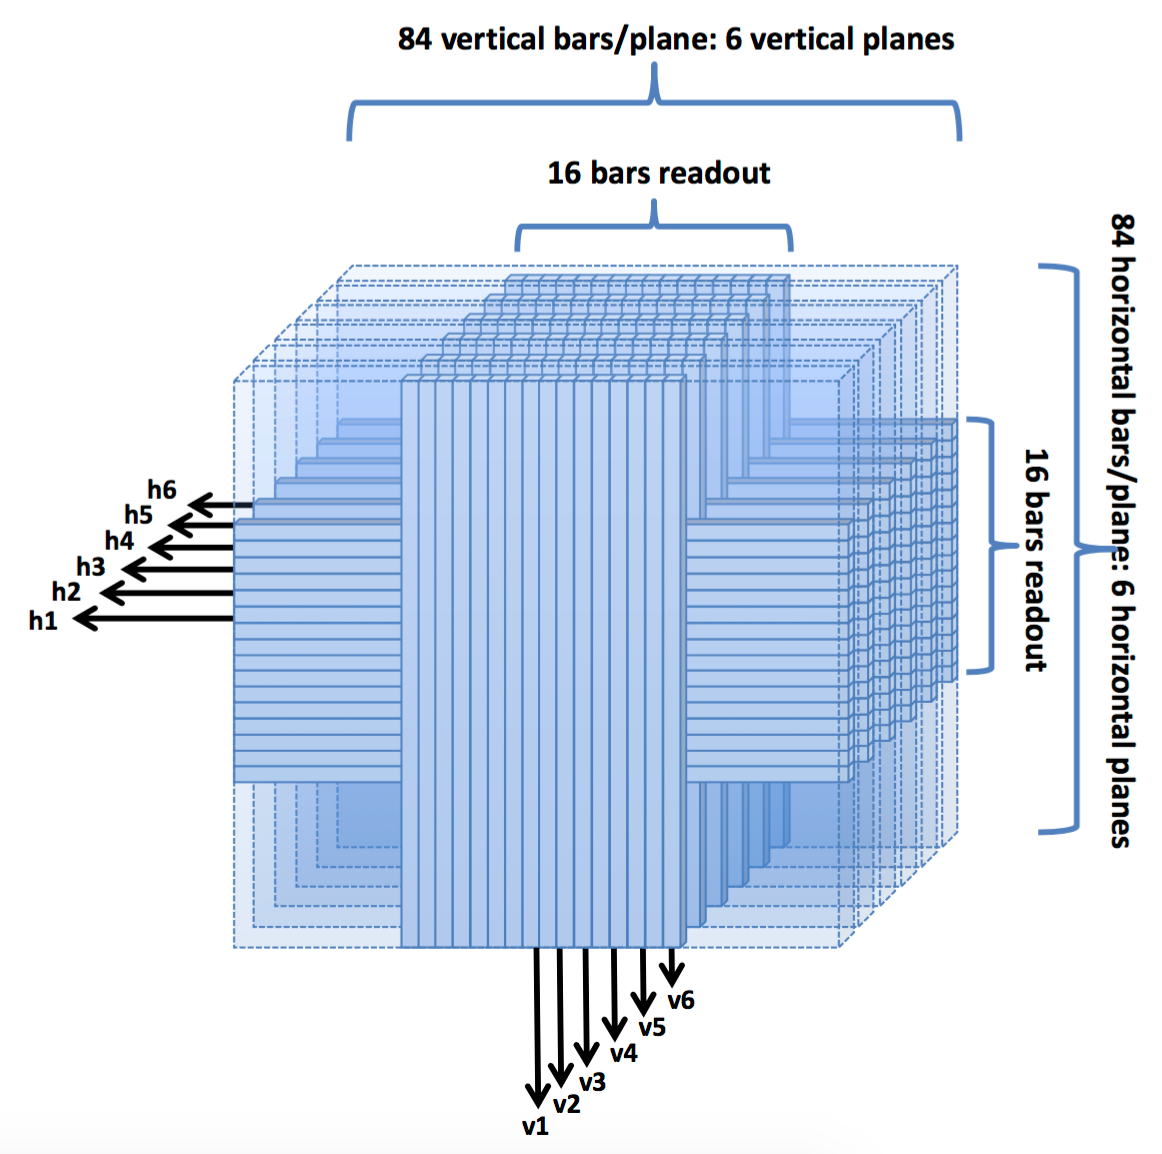
\includegraphics[width=\textwidth]{figures/AIDA.png}
\caption{The TASD with the instrumented bars visualised}
\label{fig:TASD}
\end{figure}

\begin{figure}[h!]
\centering
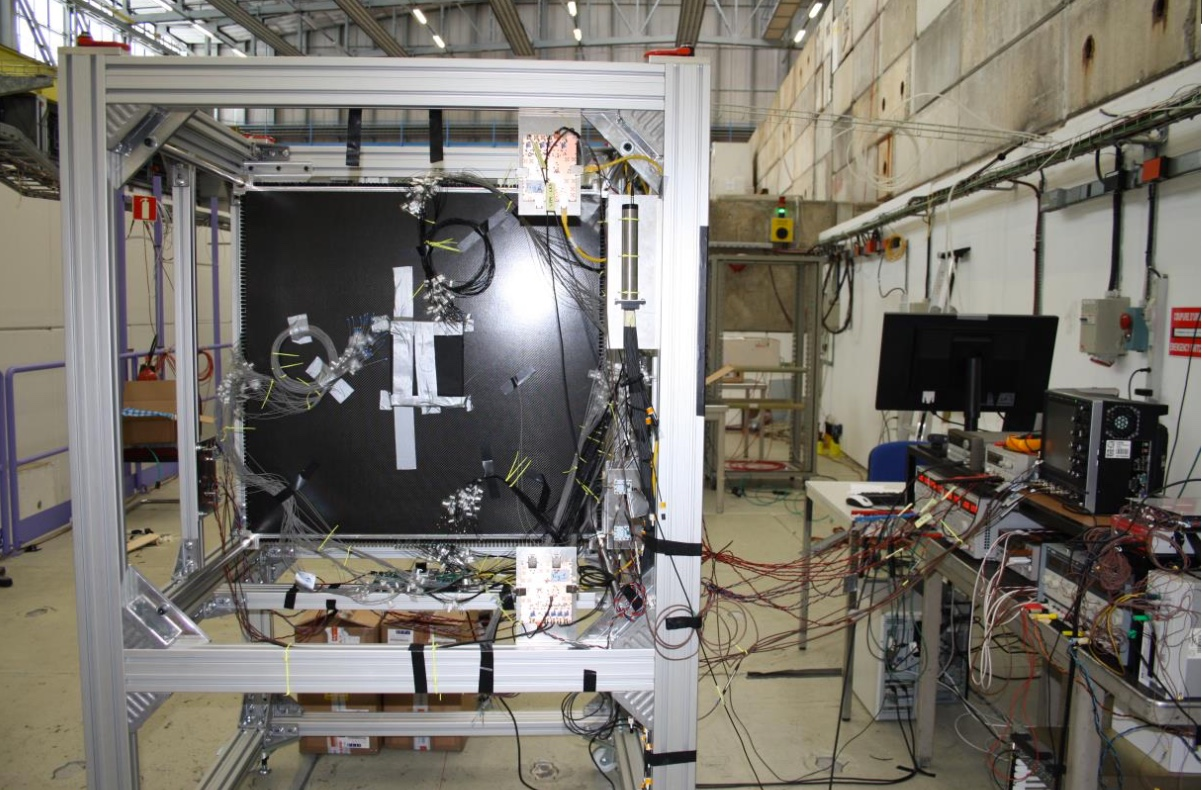
\includegraphics[width=\textwidth]{figures/TASDinstrumented.jpeg}
\caption{The TASD at the PS with the readout PC.}
\label{fig:TASDreal}
\end{figure}

\subsection{DAQ}
Each MPPC is connected to a Front End Board (FEB) which returns data in a specific format. For the setup a full 4 FEBs were used each able to read 96 MPPC channels each. These FEBs were then all connected via USB3 to a readout PC. The readout PC:s are controlled via remote connection/ethernet by a computer outside of the beam area in the control room. The data is currently just recorded, thus all analysis needs to be handled offline. This is both consequences of the data format design and the complexity of unpacking the data.

%During the initial test beam FEBv1 was used. For, ease in finding plots, details regarding FEBv2 are going to be shown.
%\textbf{Readout format and block chart can be seen in figures? }OR \cite{71Status17}. Described above under SaRoMaN.

This data is sent from each of the FEBs in a custom made data format. The data format simplifies combining the data from all of the FEBs, however it only works for offline processing as the footers need to be read before any processing can be done.

When this is done an unpacking software is used to translate the format to actual usable data and hits. During the first test beam conversion between channel and position was hard coded, this was later changed to a database.  

%Described in some part in Baby MIND section hint at the readout block figure and describe how data is taken.  All in beam area. Signal created from particle depositing energy in bar, bar producing photons, photons measured by MPPC. MPPC produces an electrical signal which is sent to FEB, which samples the signals each 2.5 ns in gtriggers of 0.1ms, in spills given by the accelerator signal. The FEB signals are sent to a back plane which sends the data several readout PC:s via USB.

\subsection{Data preprocessing}

The data recorded by the DAQ is translated using a database relating the channel number directly to a relative position for the bar as well as passing on the time of the hit. For this initial test beam there was no conversion possible between signal to deposited energy.

It was possible for the DAQ to return hits without a time which were removed before the analysis, also events which were to large time outside of the initial hit were removed.

\subsection{Results}

The main goal of this first test beam was to test the readout system, electronics, DAQ and reconstruction software. The results can be quite nicely summed up in \FigRef{fig:TASDres2} and \FigRef{fig:TASDres1} and noting that the TASD was horizontally aligned but the beam was slightly off-center vertically. Detailed studies of the electronics were performed and published in~\cite{52Georgi}.


\begin{figure}[h!]
\centering
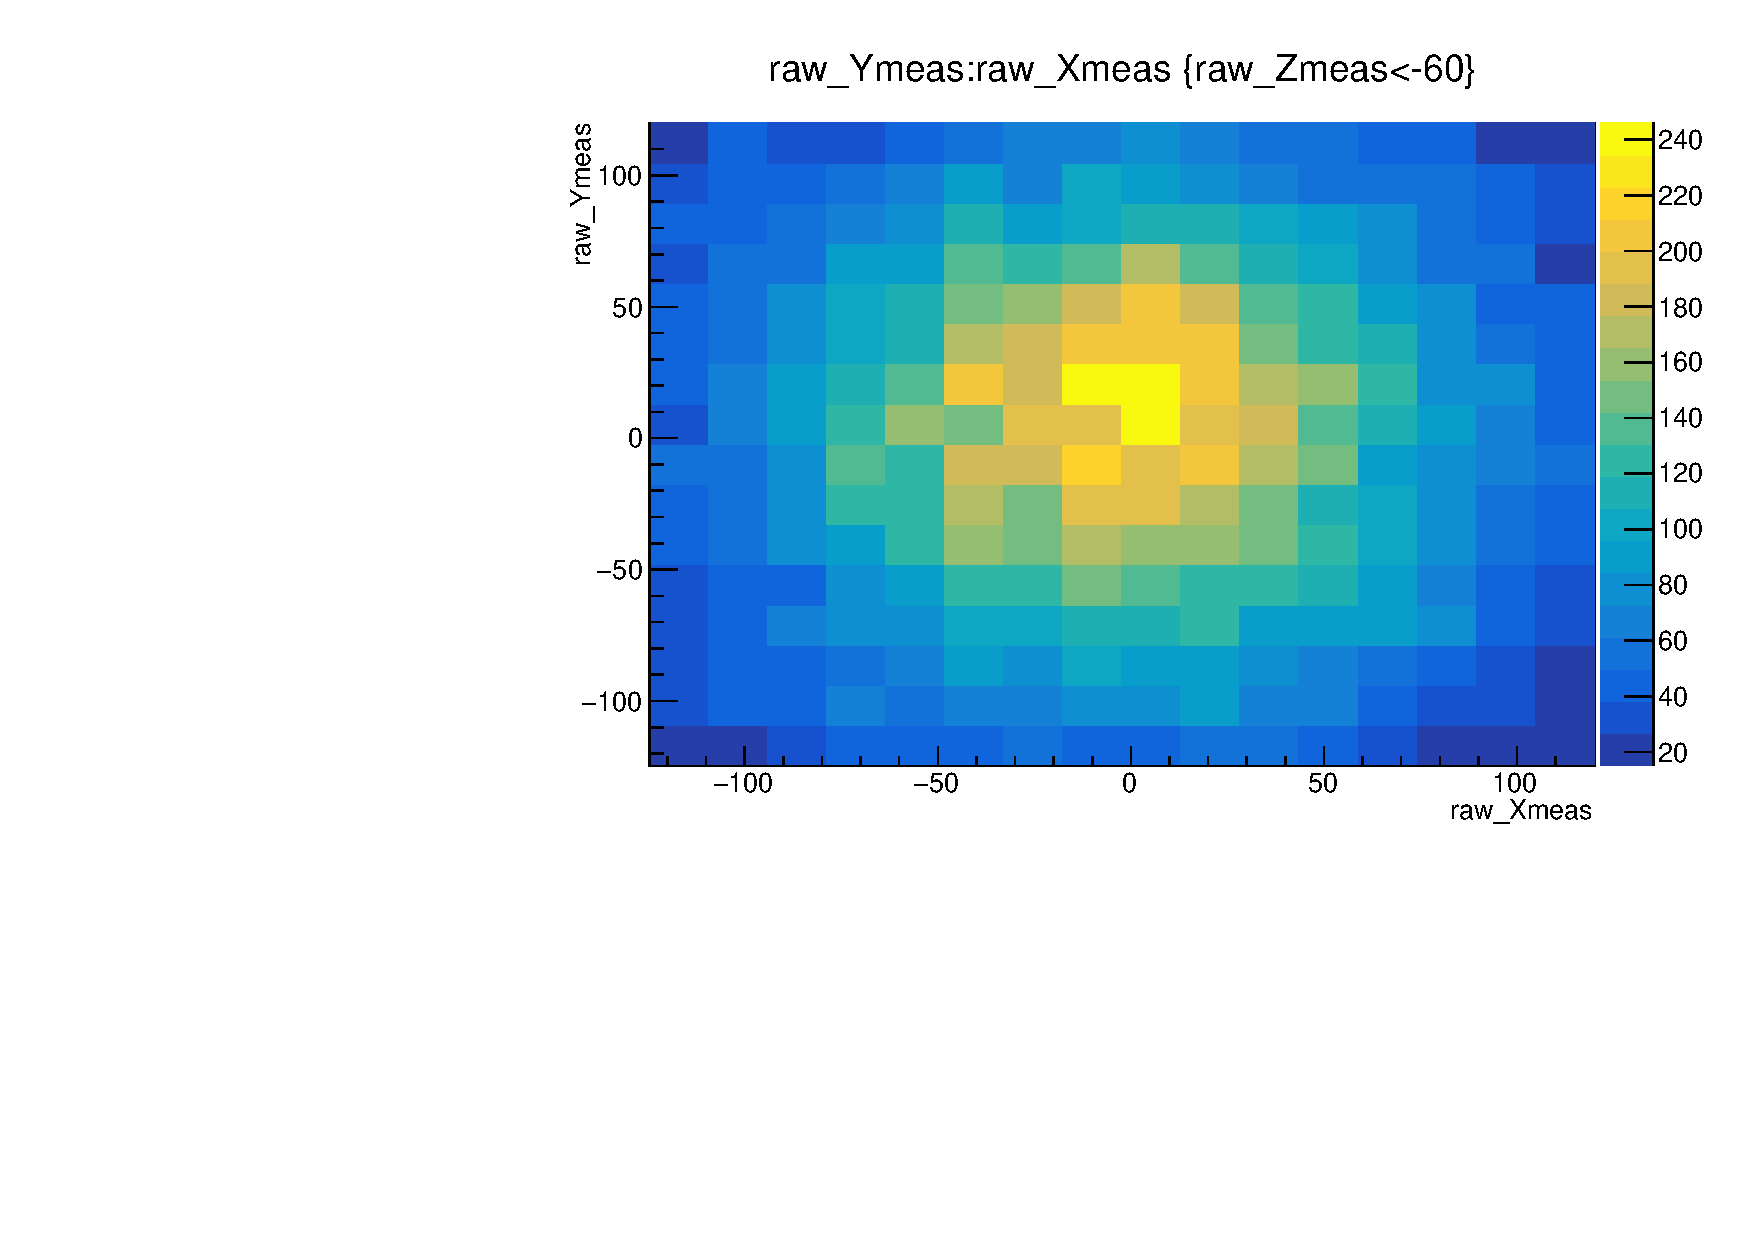
\includegraphics[width=0.48\textwidth]{figures/nuphys/newFigures/beamXYplane1Hadron.pdf}
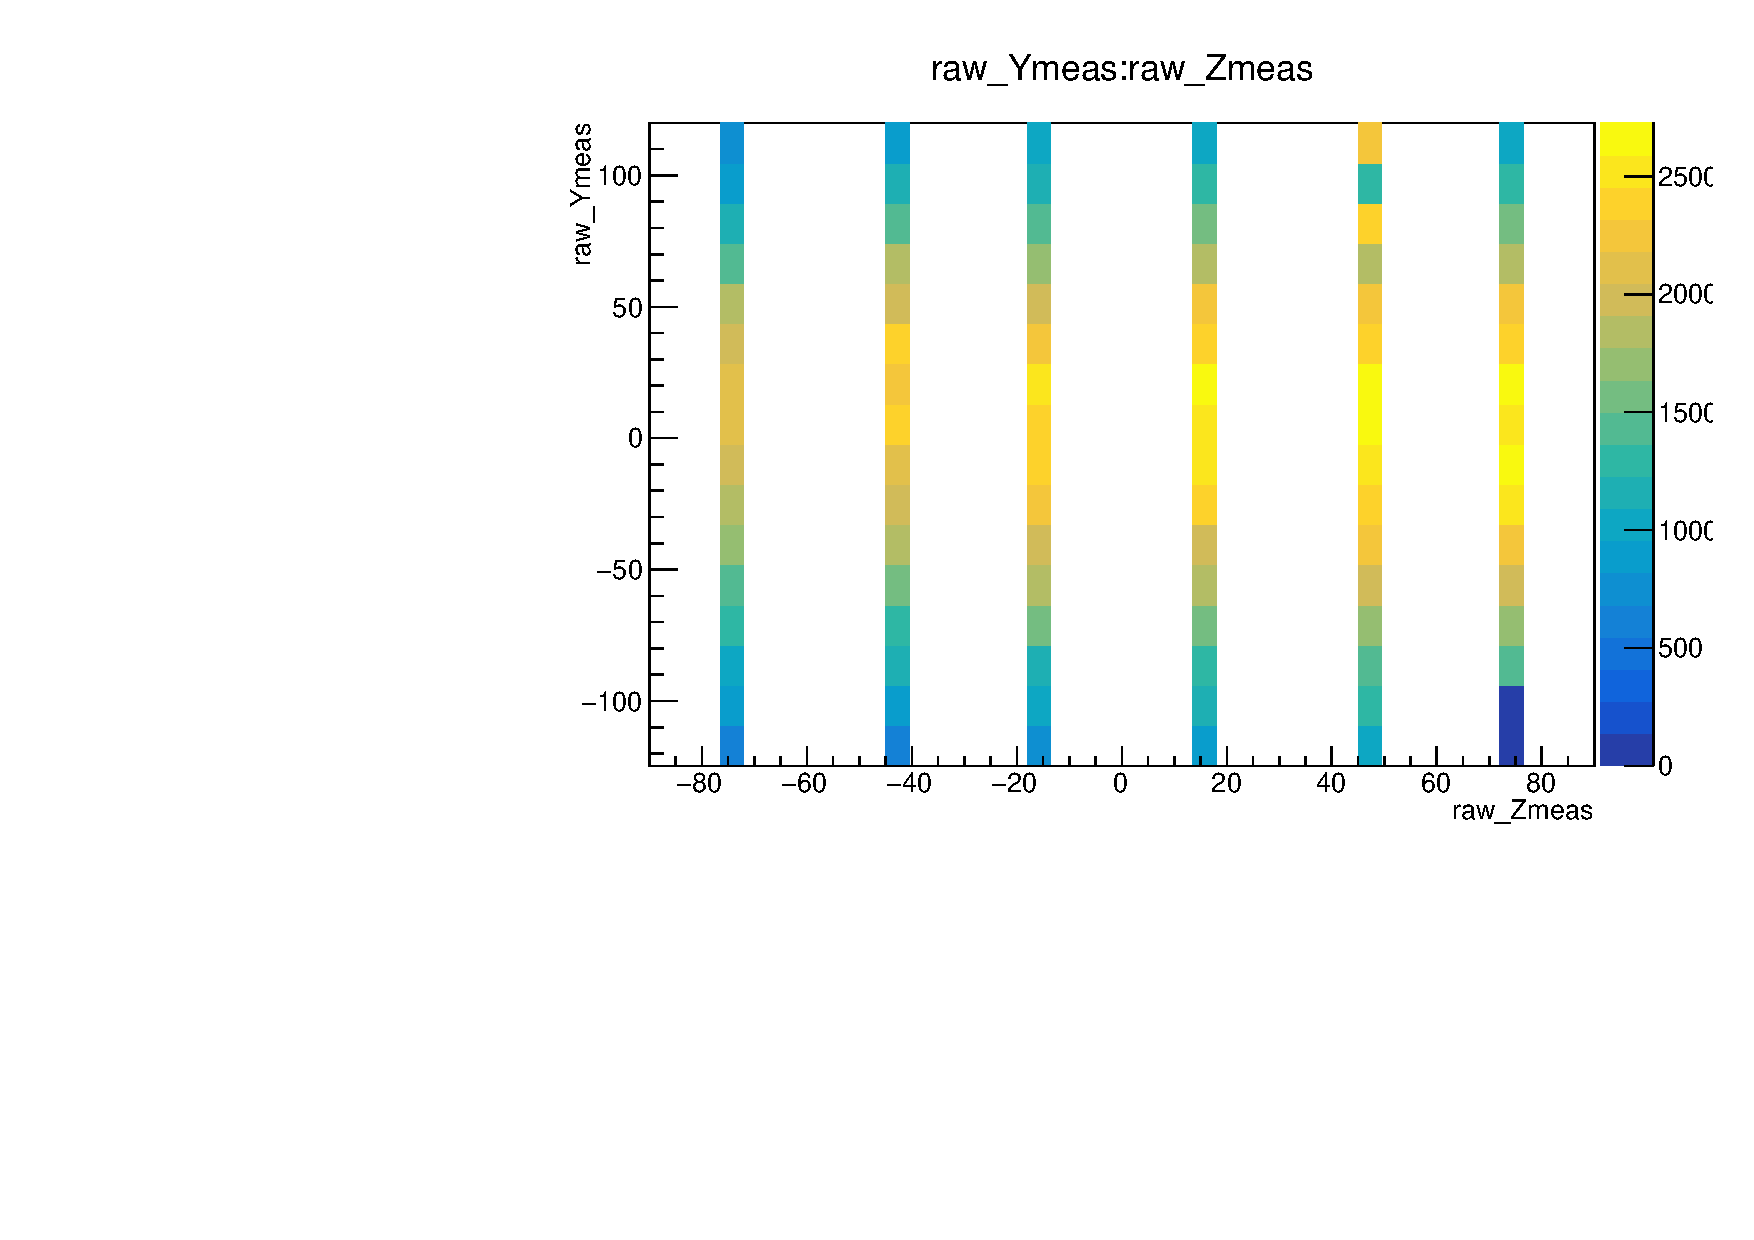
\includegraphics[width=0.48\textwidth]{figures/nuphys/newFigures/beamYZhadron.pdf}
\caption{(Left) An XY-beam profile as measured by the TASD. (Right) An YZ-beam profile as measured by the TASD}
\label{fig:TASDres2}
\end{figure}

\begin{figure}[h!]
\centering
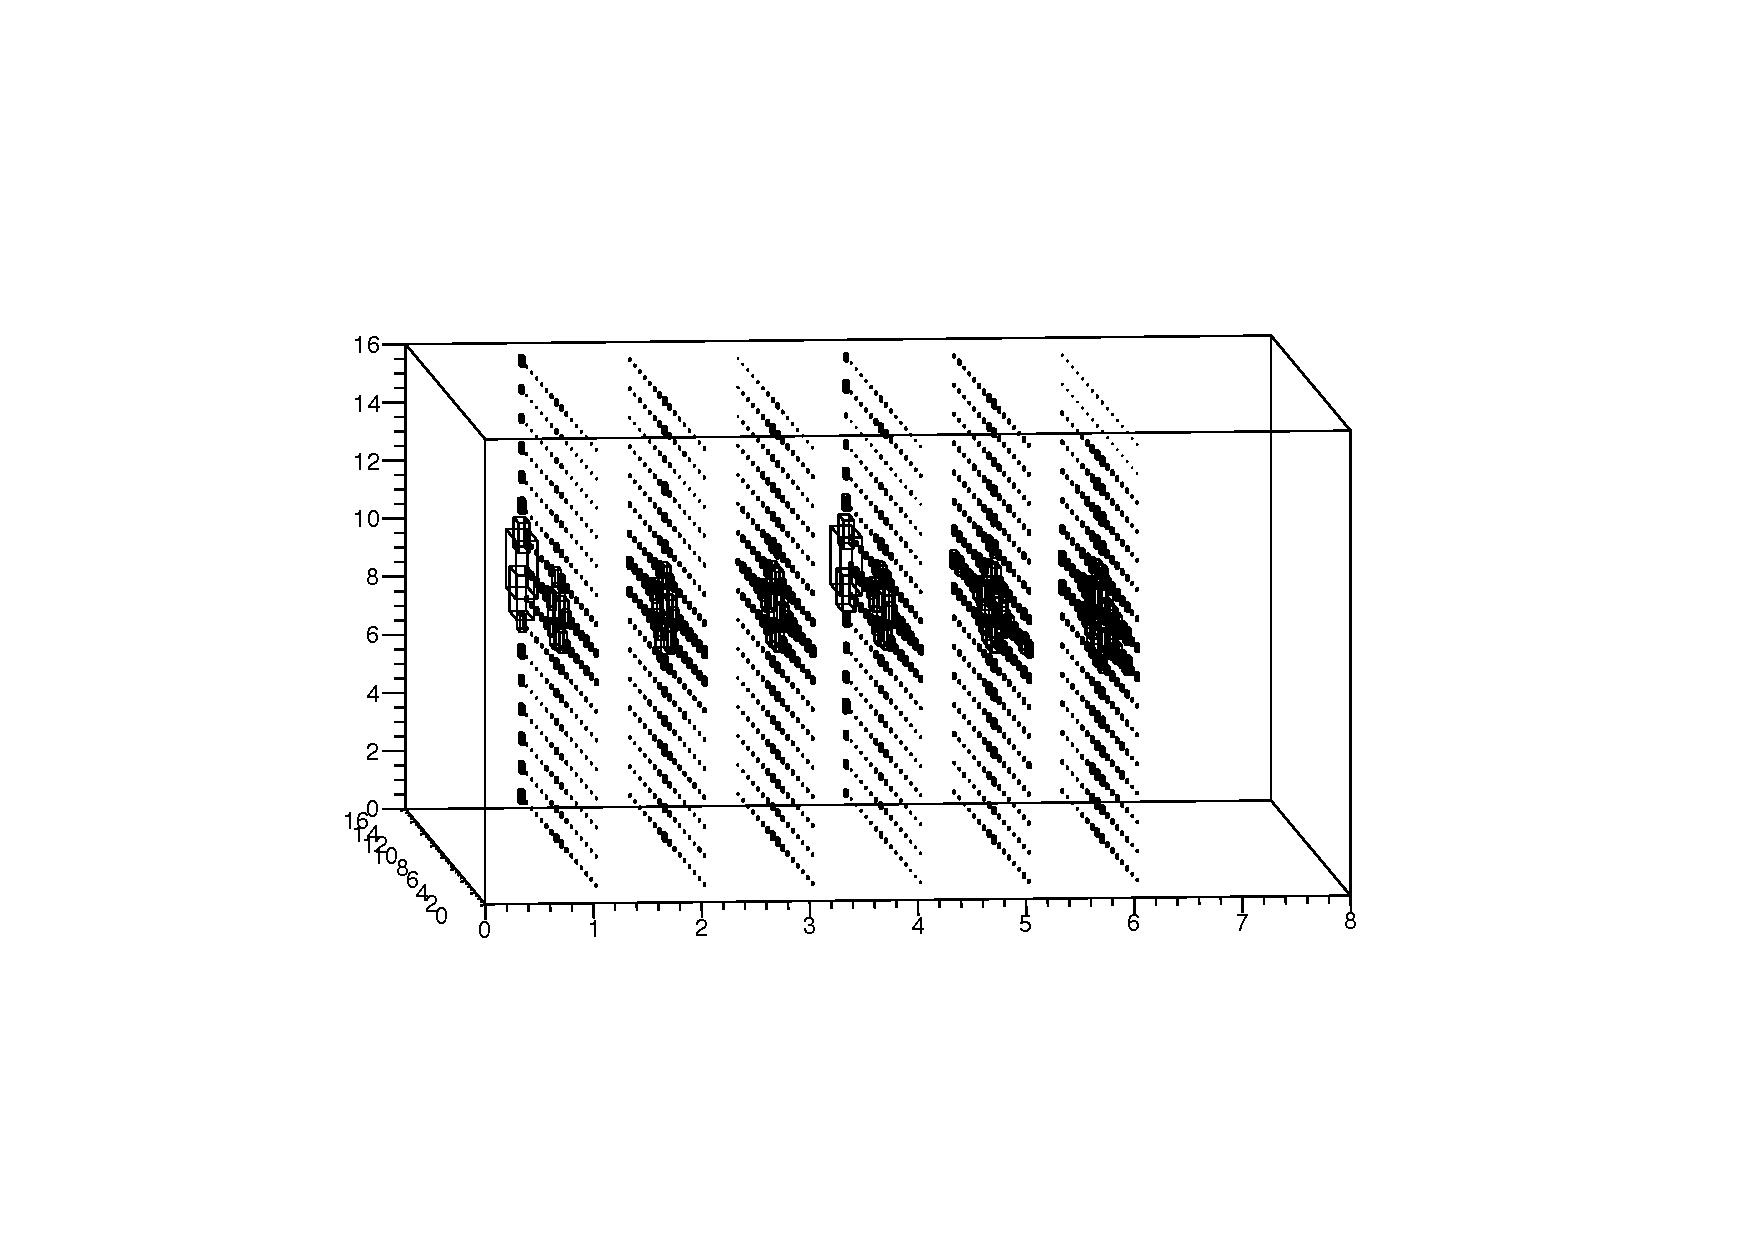
\includegraphics[width=0.48\textwidth,trim = 5cm 5cm 5cm 5cm]{figures/nuphys/newFigures/beamPlot.pdf}
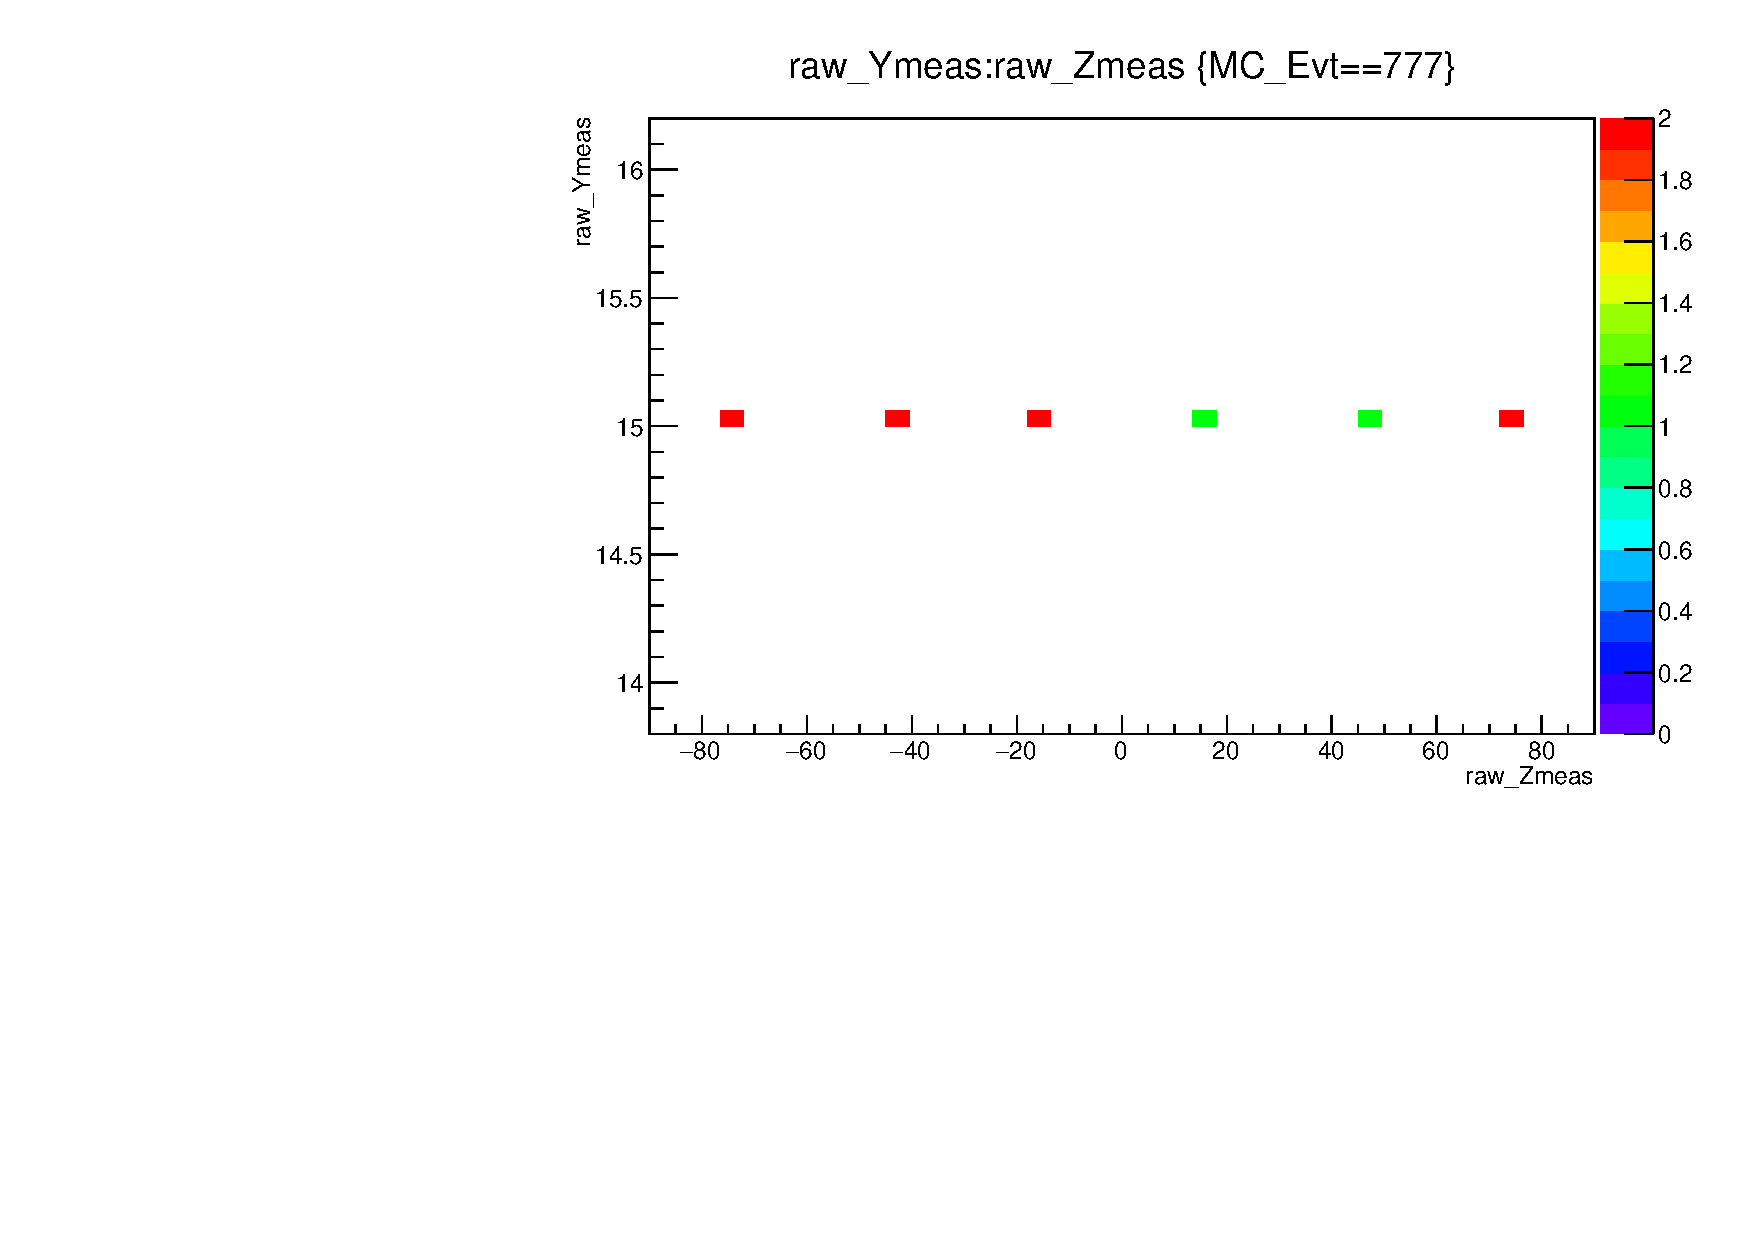
\includegraphics[width=0.48\textwidth]{figures/nuphys/newFigures/muonTrackYZ.pdf}
\caption{(Left) 3D-Beam profile measured by the TASD. (Right) Single muon track passing through the detector.}
\label{fig:TASDres1}
\end{figure}

%Add in pion track?

%What was lowest energy recorded in a bar? Results in lowest energy for horizontal and vertical.

The plots show both that the electronics and readout system works well, and that the data can be passed through the DAQ into the reconstruction software. Given that the TASD was only 6 planes of scintillator and did not have a magnetic field, the reconstruction software only combined hits in x and y with the z position to a final track, without being able to perform any momentum reconstruction. However it showed that the reconstruction software was operational and could create tracks from these hits.

%Too few planes. No magnetic field. Confirms that the full chain works and can produce plots, however the results are slightly less than expected. Add in event displays. Something to show both pion showers and muons.

%What were the results, showed that the software seems to work, both digitisation and reconstruction. Anything else? All the electronics etc. Only result from me, plots on poster...  However this shows that software works well, compared slightly to simulations??? On hardware side, daq and full chain huge improvements. Went from nothing to ensuring that bars work properly (done previously) show that FEB reads out data and that this is passed to computer. DAQ can then use this to unpack the data correctly and finally into SaRoMaN for visualization.

\pagebreak
\section{MIND-test beam}

The Baby MIND qualification took place at the T9 beam line at the PS experimental hall (East Area), during June - July 2017. The beam lines are derived from the 24 GeV/c primary proton beam from the PS, which provides 2.4 s cycles of about 400 ms spill duration. The T9 beam is a secondary beam from the collision of the proton beam with a 200 mm thick Aluminium target, that delivers secondary particles up to 15 GeV/c at a production angle of 0 degrees. The line is designed to provide the users with non-separated secondary particles, with positive or negative polarity. Users can adjust the beam momentum by setting the currents for the optical magnets of the beam line. A sketch of the layout can be seen in~\FigRef{fig:MINDtb} and a photograph in~\FigRef{fig:MINDtbreal}.

\begin{figure}[h!]
\centering
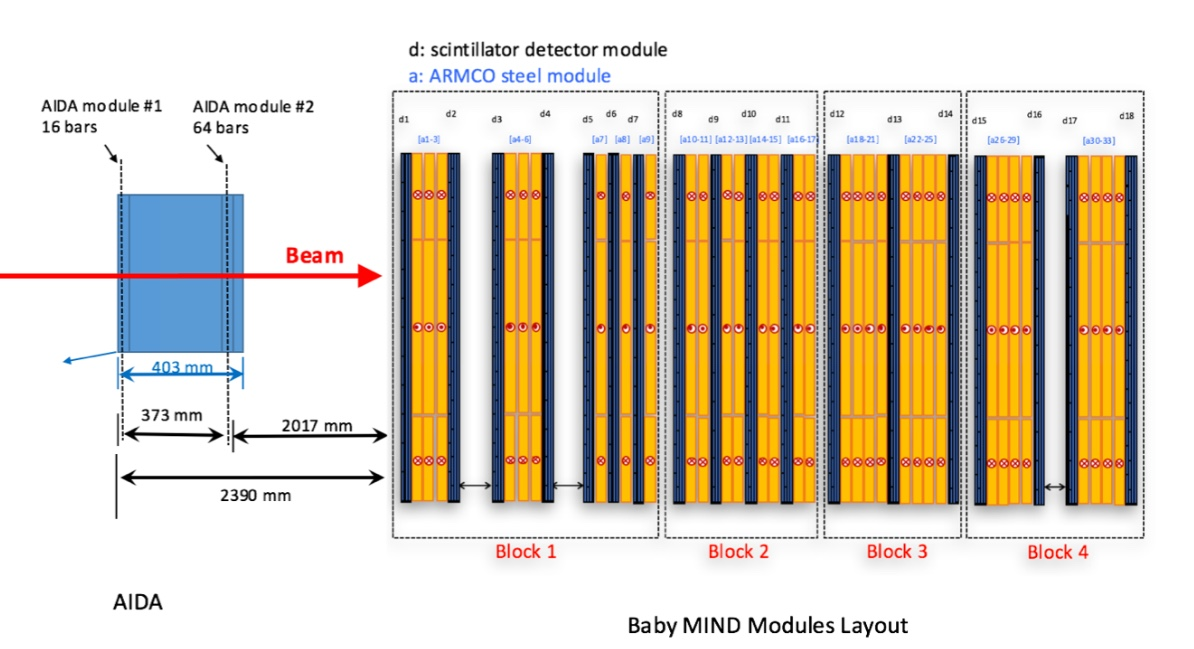
\includegraphics[width=\textwidth]{figures/MINDAIDAtestbeam.jpeg}
\caption{MIND in testbeam.}
\label{fig:MINDtb}
\end{figure}

\begin{figure}[h!]
\centering
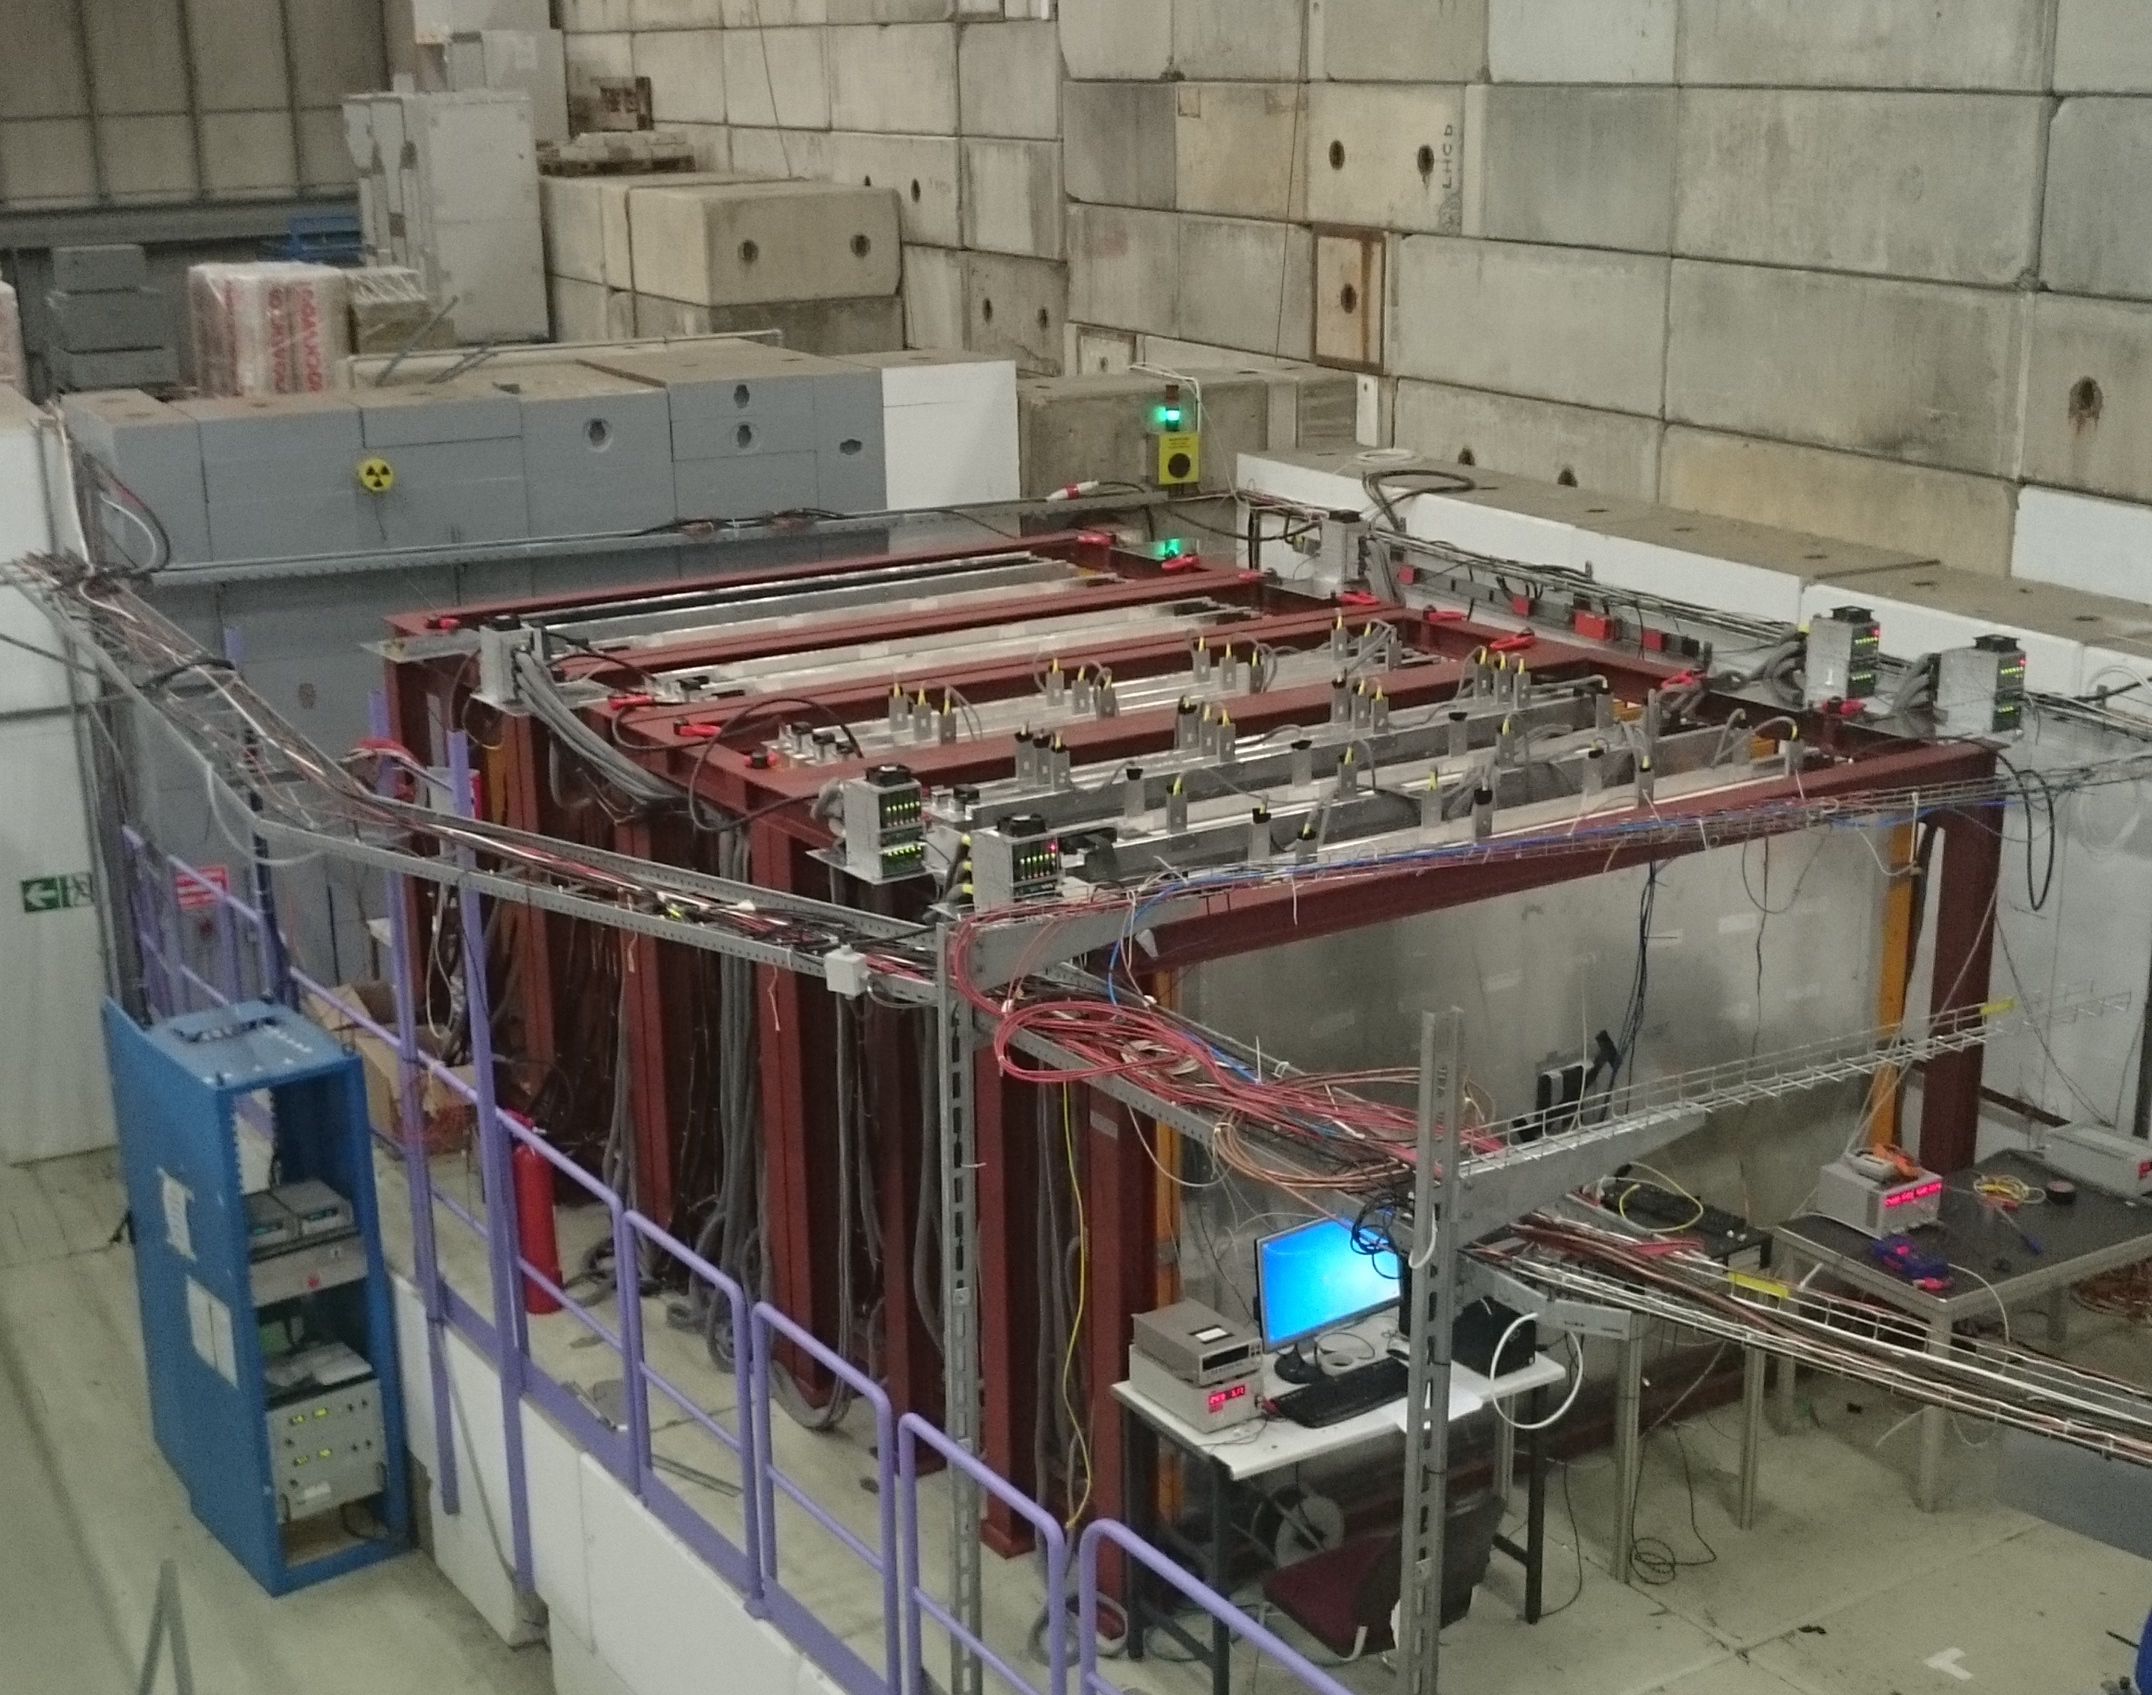
\includegraphics[width=\textwidth]{figures/DSC_2619.JPG}
\caption{MIND in testbeam photo.}
\label{fig:MINDtbreal}
\end{figure}

\subsection{Setup}

In order to support the magnets and scintillating modules mechanically, four support frames were constructed specifically to support the Baby MIND and  to meet the transport requirements within CERN and shipping to J-PARC. The Baby Mind modules were installed in the four frames. The total weight of the detector is around 65 t giving each block a weight of at less than 20 tons which is within the required limits for crane operations at both sites.

For the data taking during the test beam, the TASD was placed in front of the Baby MIND to provide initial beam information, both an angular measurement of the beam and a veto measurement from cosmic rays. Only a total of 2 planes of the TASD were instrumented providing 192 channels. 

A total of 44 FEBs mounted on 8 mini crates instrumented the 3996 channels of Baby MIND and took the 192 channels from the TASD. All 44 FEBs were synchronized using the spill signal from T9 beam line which arrives one second before the arrival of the spill of particles. This signal was fed to a dedicated Master FEB which would generate a reference clock signal for all the other FEBs acquiring data.

\subsection{Data preprocessing}
The data recorded by the DAQ is translated using a database relating the channel number directly to a relative position for the bar as well as passing on the time of the hit. For this initial test beam there was no conversion possible between signal to deposited energy.

It was possible for the DAQ to return hits without a time which were removed before the analysis. And also events which were to large time outside of the initial hit were removed.

For this test beam initial filters were used to try to removed possible pion contamination such as removing events where on average more than three hits were recorded for the same plane for an event. 

Data was taken for a period of 2 months. Out of the recorded data, a verified samples with the best possible settings for the data acquisition was selected for analysis. The samples contained a few hours worth of data taking at different beam momenta for both muons and anti-muons beam settings. These samples were all run through the unpacking software required to read out the recorded data before being passed to SaRoMaN. The data was passed directly into the digitisation for clustering and grouping before being passed into the reconstruction..

\subsection{Analysis}

For the first part of the analysis the data sample was assumed to be quite clean, containing mostly only muons or anti-muons. To remove any contribution from outside of the beam the hits in the TASD were used as a beam trigger to defined a time window of  interest from this time and 125 ns after and used to fit any tracks. This time was chosen after seeing what was appropriate for our data structure. To remove any potential showers or noise any event less than 4 hits in MIND or on average more than 10 hits per plane were removed.

Data was run through the SaRoMaN software framework and produced plots of charge reconstruction efficiency, momentum reconstruction etc etc and compared to simulations.

In the analysis it was also quite clear that the beam was not pure muons and contained some contamination of other particles. The main contamination seems to be pions. Thus for the second analysis the data was firstly run through a TMVA software packages providing many different machine learning techniques which would perform the particle identification of muons vs pions.



%Talk about different samples, event selection.
%Initially started with data recorded under x amount of hours. This is then passed through the the reconstruction ...
%TMVA used....


%Compare momentum and spread. Mention that filters could be used to improve data. Momentum comparison, unknown real true momentum and particle ID. TMVA used to try to see if possible to separate and identify particle type. Describe also how it was trained, mention in section 4.

%Show perhaps possibility in looking at single track events to identify showers vs muonlike particles. Also can see curvature and make an initial momentum guess based on it or based on the range if the event stops in the detector.


\subsection{Results}
Two of the main results provided during the test beam were both to commission the detector by showing that all parts works, including the reconstruction framework with hits in all of the modules, and magnetic field providing the ability to estimate momentum. Results will be presented showing that the detector has been commissioned and showing that the reconstruction framework can read in this data and produce charge and momentum estimates for the beam.

\subsubsection{Electronics results}

Gain plots for all of the 3996 MPPCs installed on Baby MIND. The gain is evenly distributed around 45 ADC/photoelectrons $\pm  5$ as seen in \FigRef{fig:MPPCplot1}. This can be further improved by optimising the pre-amp gain on the FEB for each of the MPPCs.

\begin{figure}[h!]
\centering
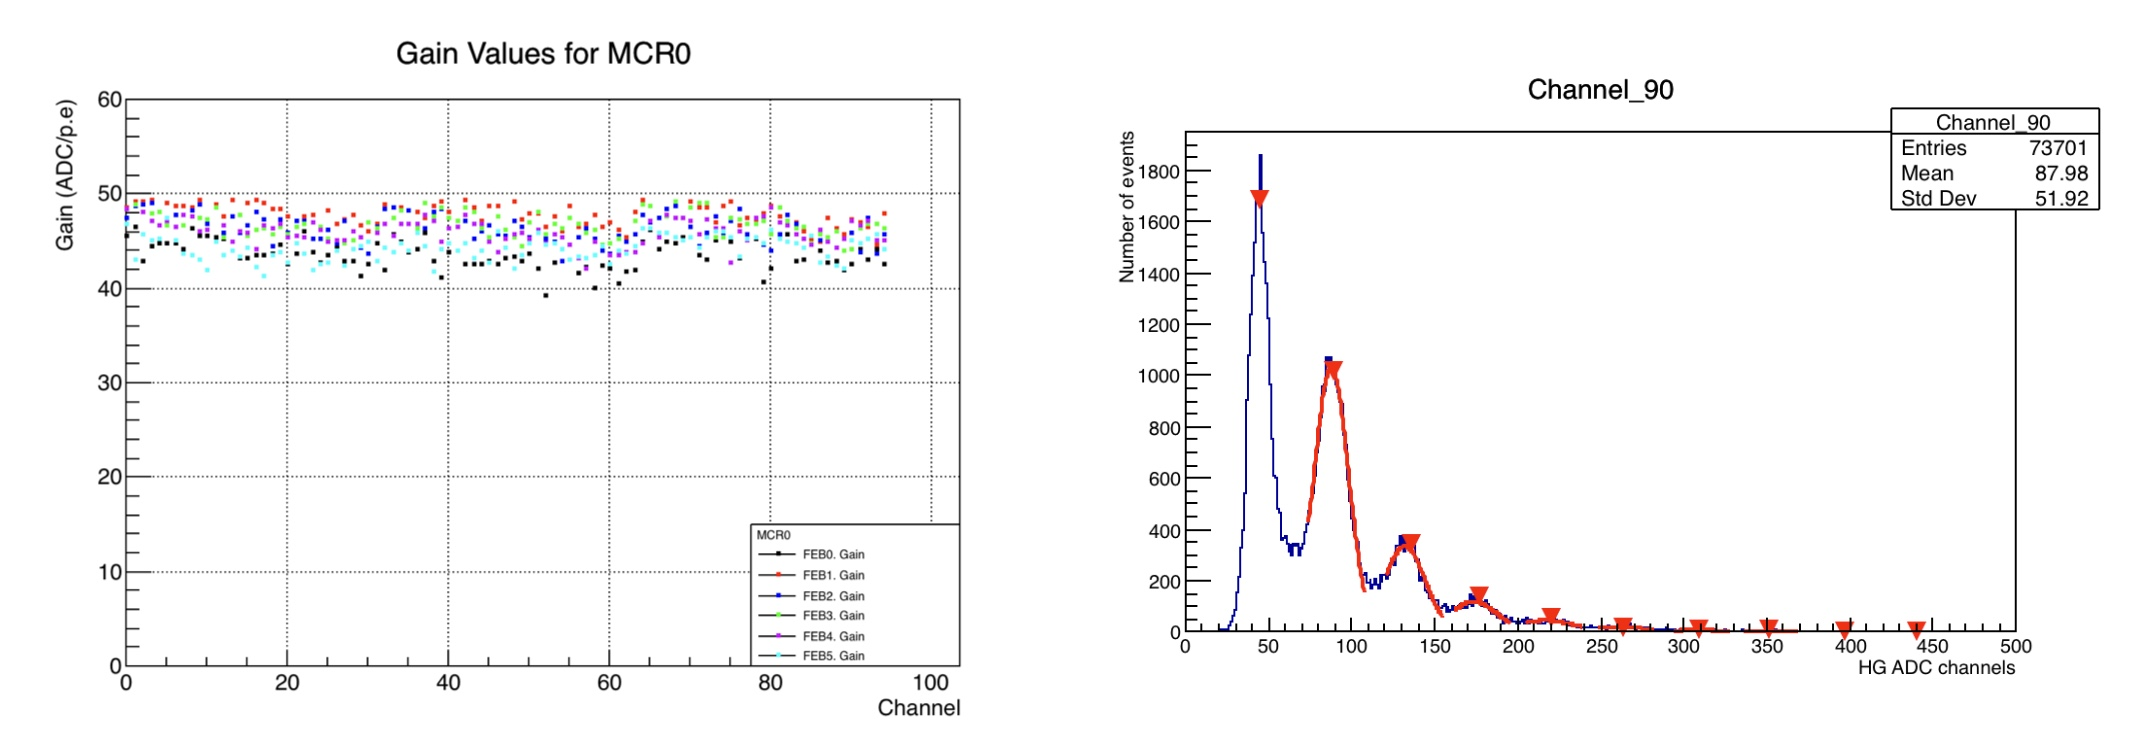
\includegraphics[width=\textwidth]{figures/mppcplot1.jpeg}
\caption{Gain for 576 channels (left) and noise spectrum finger plots with 5 viable peaks.
 for one channel (right).}
\label{fig:MPPCplot1}
\end{figure}

\subsubsection{Magnet results}

The magnet performance was measured at CERN, with detailed tests on the first module allowing comparisons verification of simulations. The magnet modules reached the design specification of 1.5 T for a current of 140 A. Stray fields were measured at $<10$ mTat a distance of 1 mm from the surface of the magnet modules. The measured power consumption at CERN was 11.5 kW. %The measured power consumption at J-PARC is 11.1 kW. The ambient temperature at J-PARC is 10C lower which accounts for the lower aluminium coil temperatures and resistances. 
The current and voltage reach stable operating values several hours, this can be seen in~\FigRef{fig:Magnetplot1}.

\begin{figure}[h!]
\centering
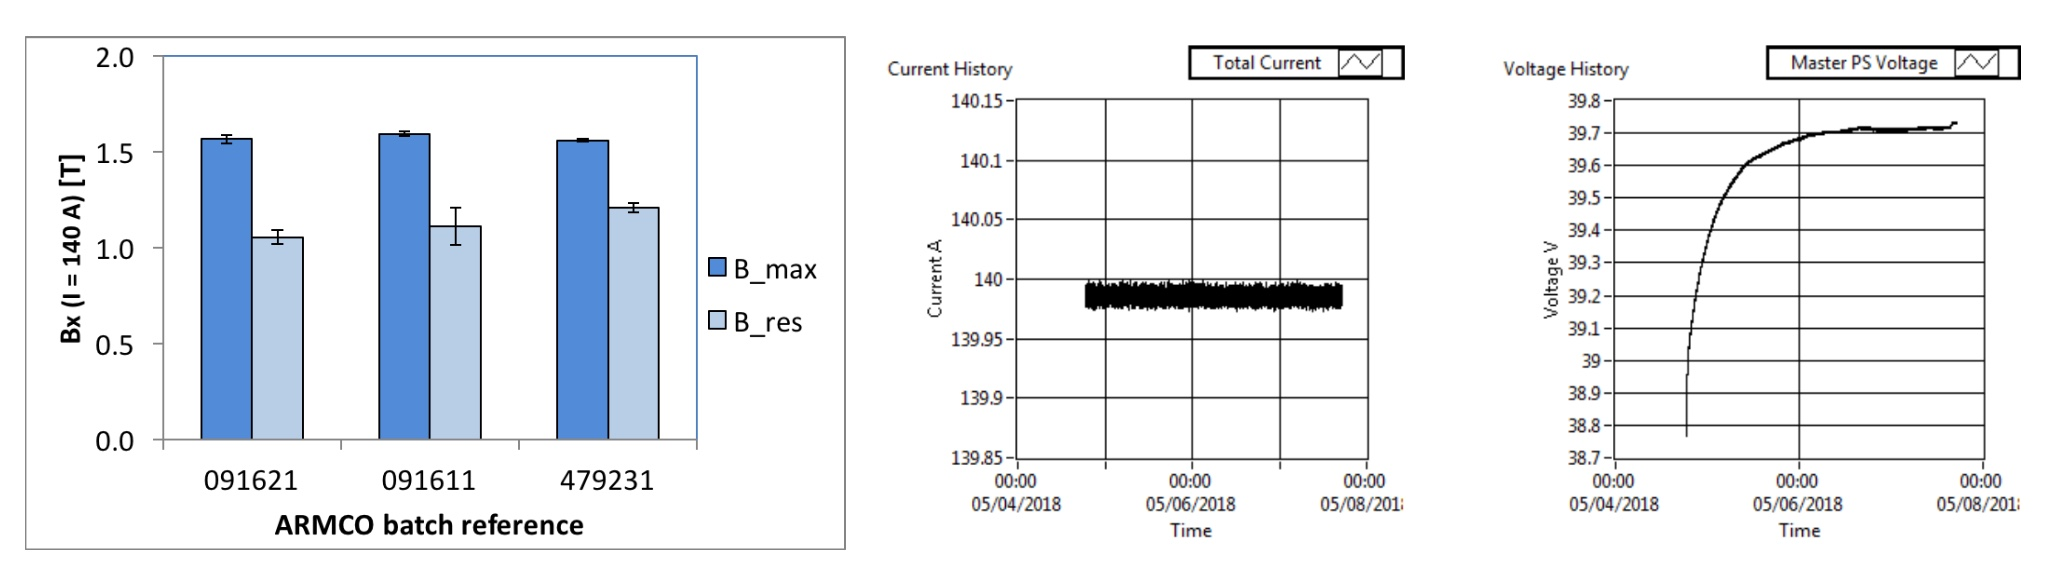
\includegraphics[width=\textwidth]{figures/magnetFigure1.jpeg}
\caption{Baby MIND magnet measured (at CERN) field values for 33 modules (left), current at J-PARC (middle) and corresponding voltage (right).}
\label{fig:Magnetplot1}
\end{figure}



\if{0}
\subsubsection{Data from unpacking}
Low level hits from only unpacking.

\subsubsection{Tracks from unpacking}
Using this data to build tracks.
\fi

\subsubsection{Hits in SaRoMaN}
Using the recorded data, the SaRoMaN needed to be verified to see if it could combine the bar data into 3D space points. As can be seen in \FigRef{fig:hitmap} the planes show up well with no obvious missing hits and a similar filling of hits on all planes.

\begin{figure}[h!]
\centering
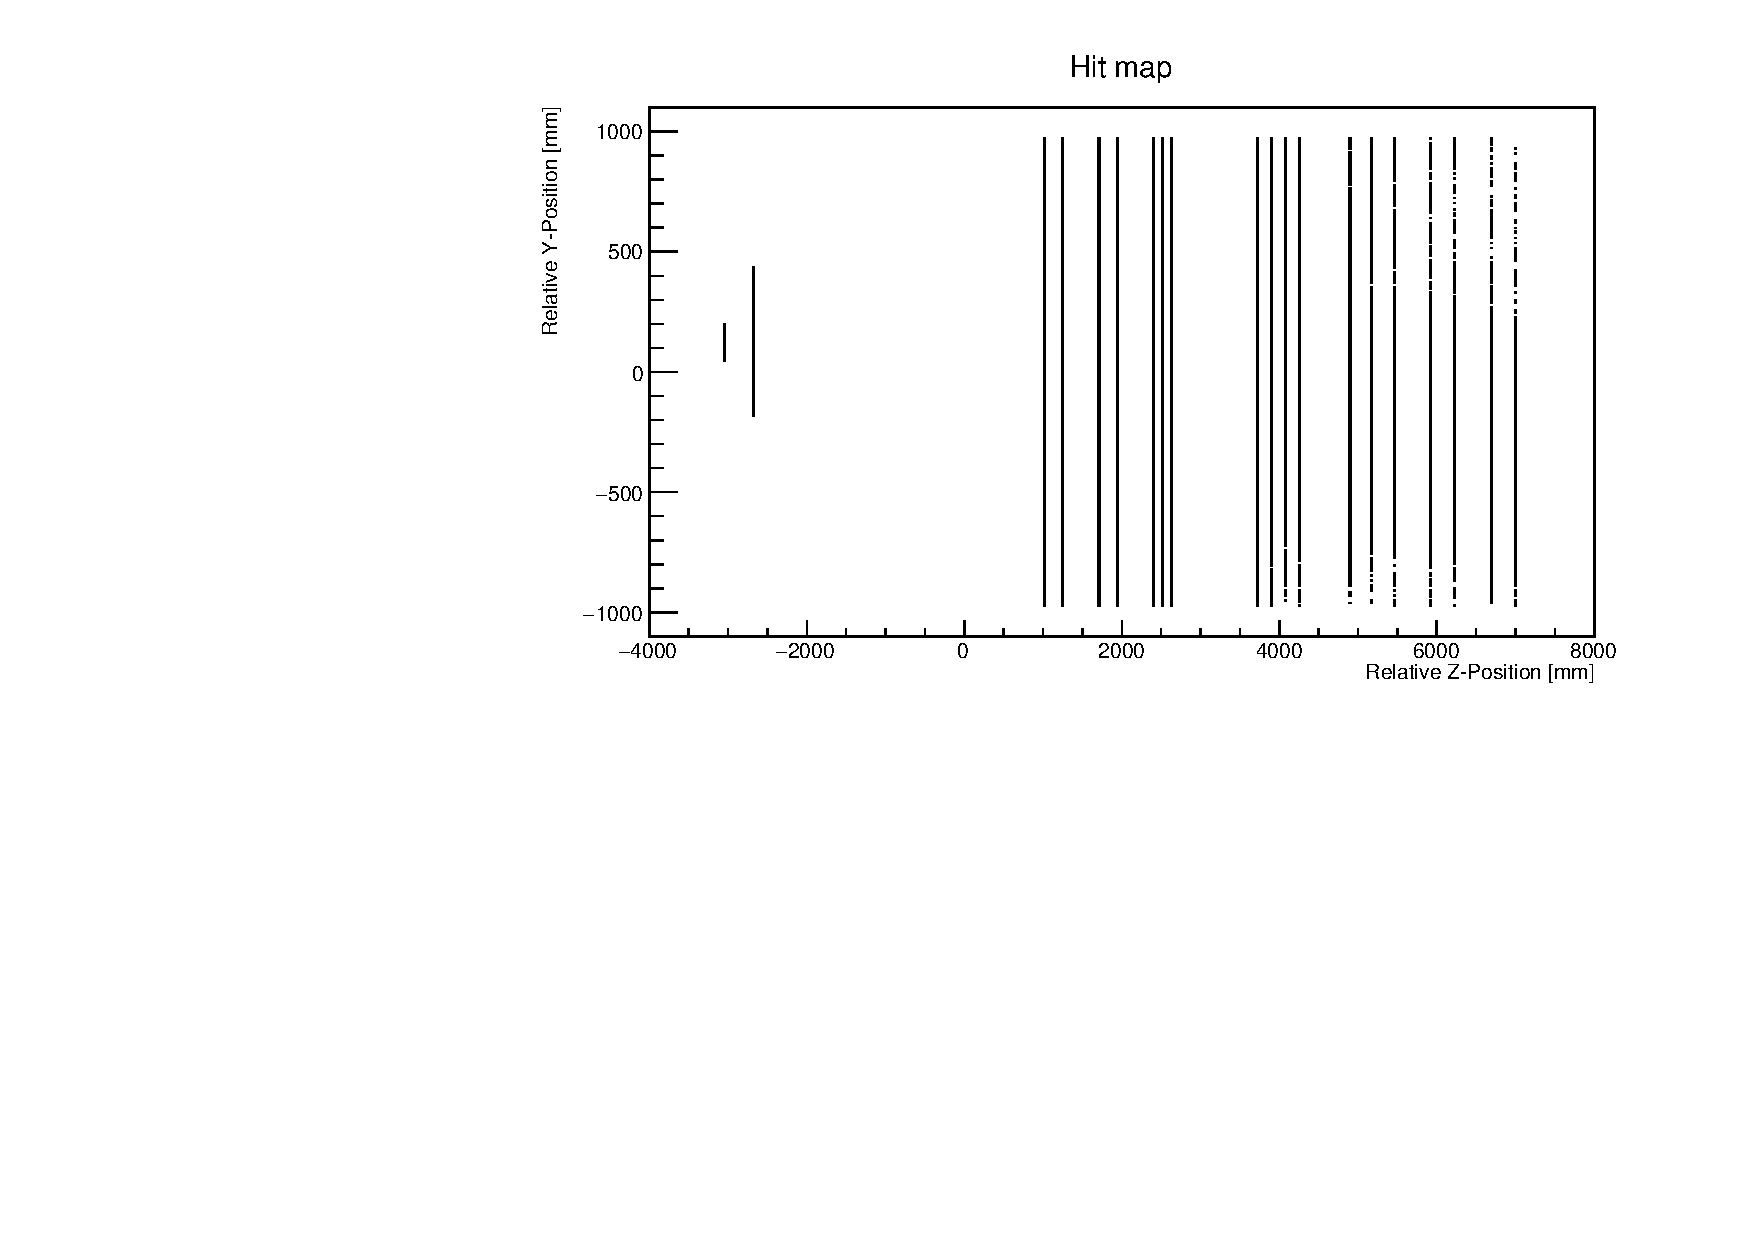
\includegraphics[width=\textwidth]{figures/HitMap5GeVYZ.pdf}
\caption{All recorded hits for a run with the 5 GeV beam settings.}
\label{fig:hitmap}
\end{figure}


\subsubsection{Tracks in SaRoMaN}
In a similar way to simulated data, the collected hits are split depending on the time the hits were recorded to build possible tracks, seen in \FigRef{fig:event} and \FigRef{fig:EventsInitial}. Each of these possible tracks are then filtered through to produce the best possible fitted track for those points and some background or noise hits. This can become quite complicated if there are two tracks passing through simultaneously, however this can be handed by the software even though this phenomena is rare.

The main difficulty comes from the framework only reconstructing tracks and discarding shower events. Any track reconstruction of a shower should fail, but sometimes it will try and return an incorrect charge and momentum value. This makes it clear that data of showers need to be removed before any analysis is performed by using pattern recognition to identify showers (non-muons) from muons (non-showers).

\begin{figure}[h!]
\centering
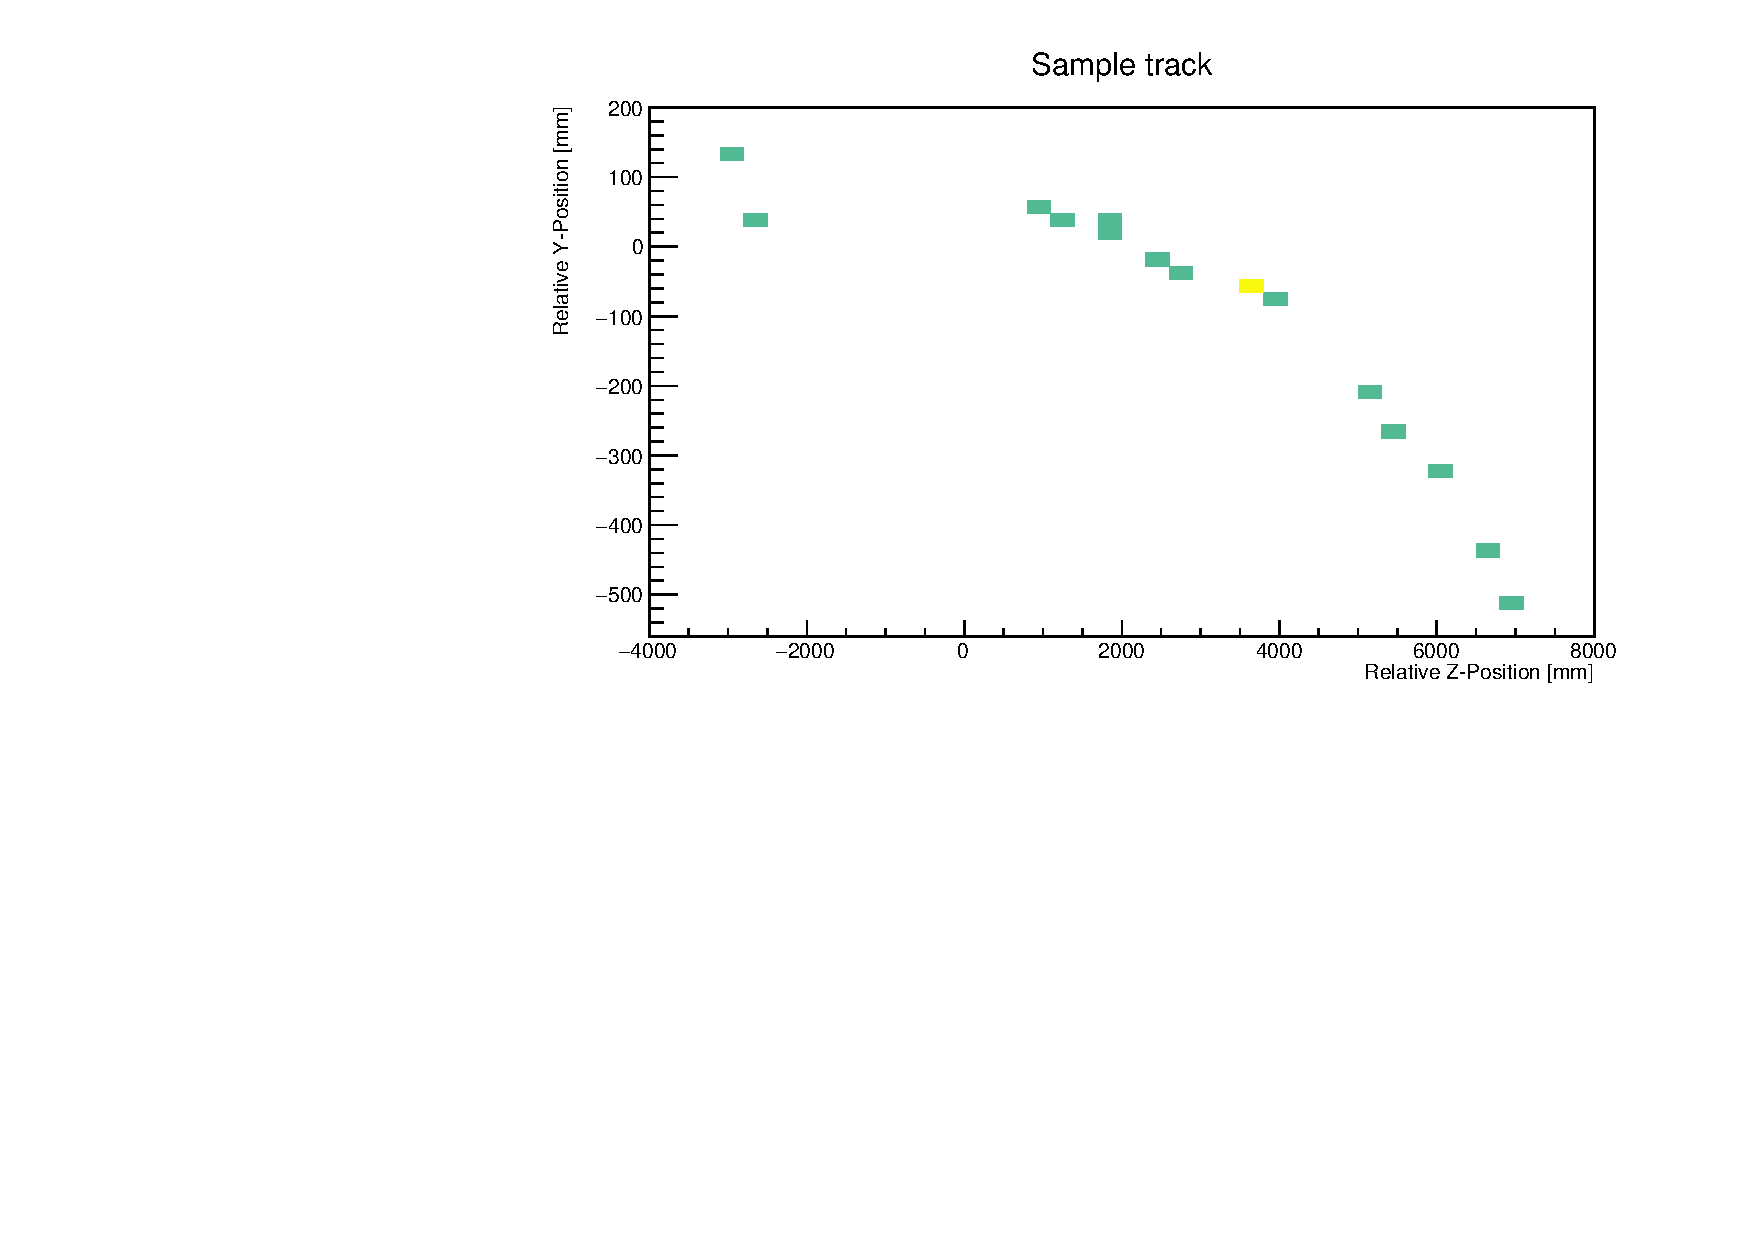
\includegraphics[width=\textwidth]{figures/SampleTrack5GeVYZ.pdf}
\caption{A sample track, taking a time cut for the hits for a run with the 5 GeV beam settings.}
\label{fig:event}
\end{figure}

\begin{figure}[h!]
\centering
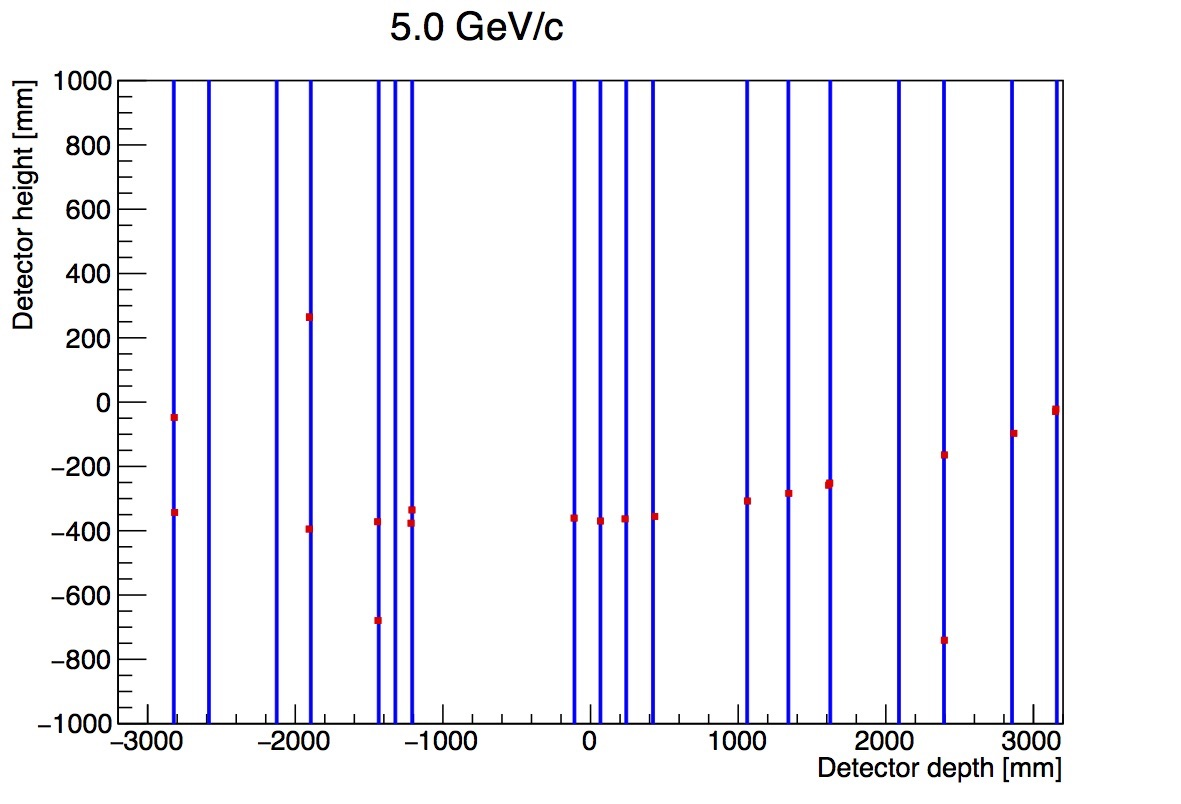
\includegraphics[width=\textwidth]{figures/oldStudies/m5GeVevent2.jpg}

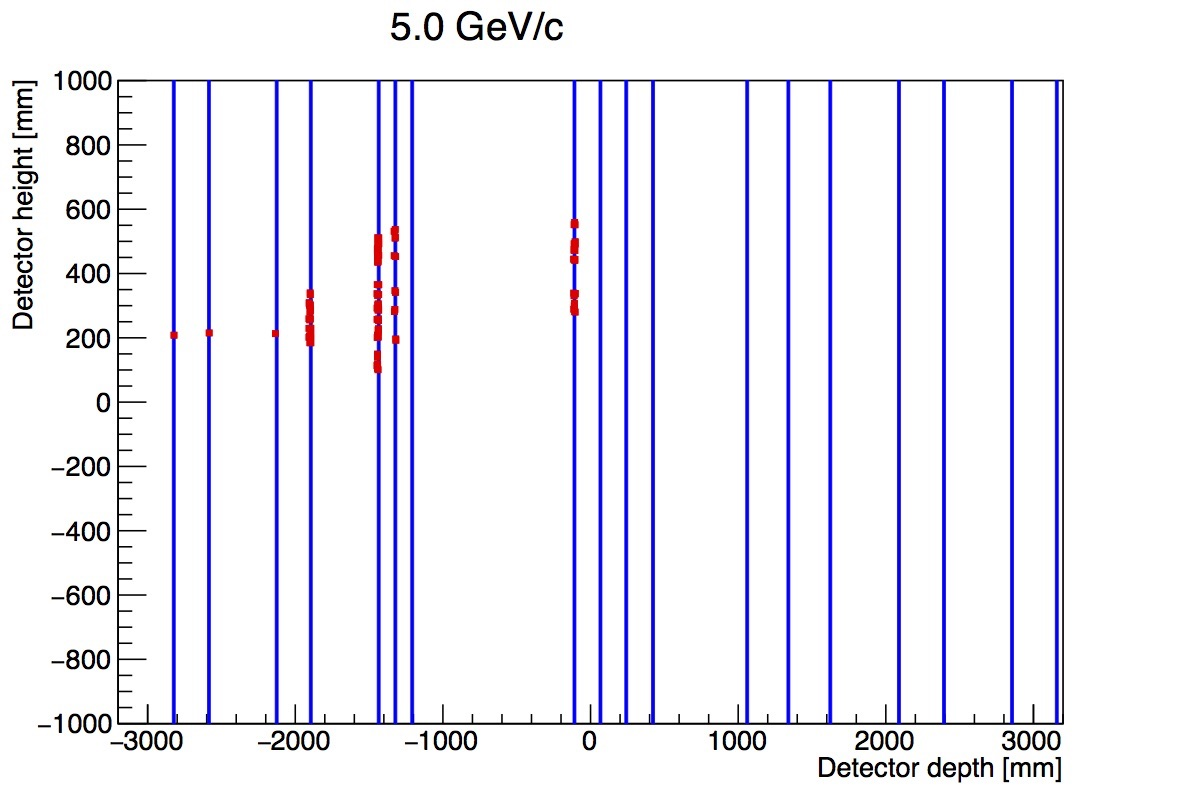
\includegraphics[width=\textwidth]{figures/oldStudies/m5GeVevent3.jpg}
\caption{Sample events of test beam interactions at a set energy value of $5GeV/c$.}
\label{fig:EventsInitial}
\end{figure}

\subsubsection{Charge identification efficiency}
One of the main goals of the Baby MIND detector is to correctly identify the charge of incoming muons. In the test beam it is difficult to estimate the number of muons produced since the beam itself is a mix of mostly muons and pions. As seen above, the reconstruction software can return the number of tracklike events against the number of reconstructible tracks. With these reconstructible tracks the charge can then be reconstructed and a charge identification efficiency plotted as seen in~\FigRef{fig:ChargeInitial}. Initial results of this study were shown at NuFact2017 and published in~\cite{82Uppsala}.


\begin{figure}[h!]
\centering
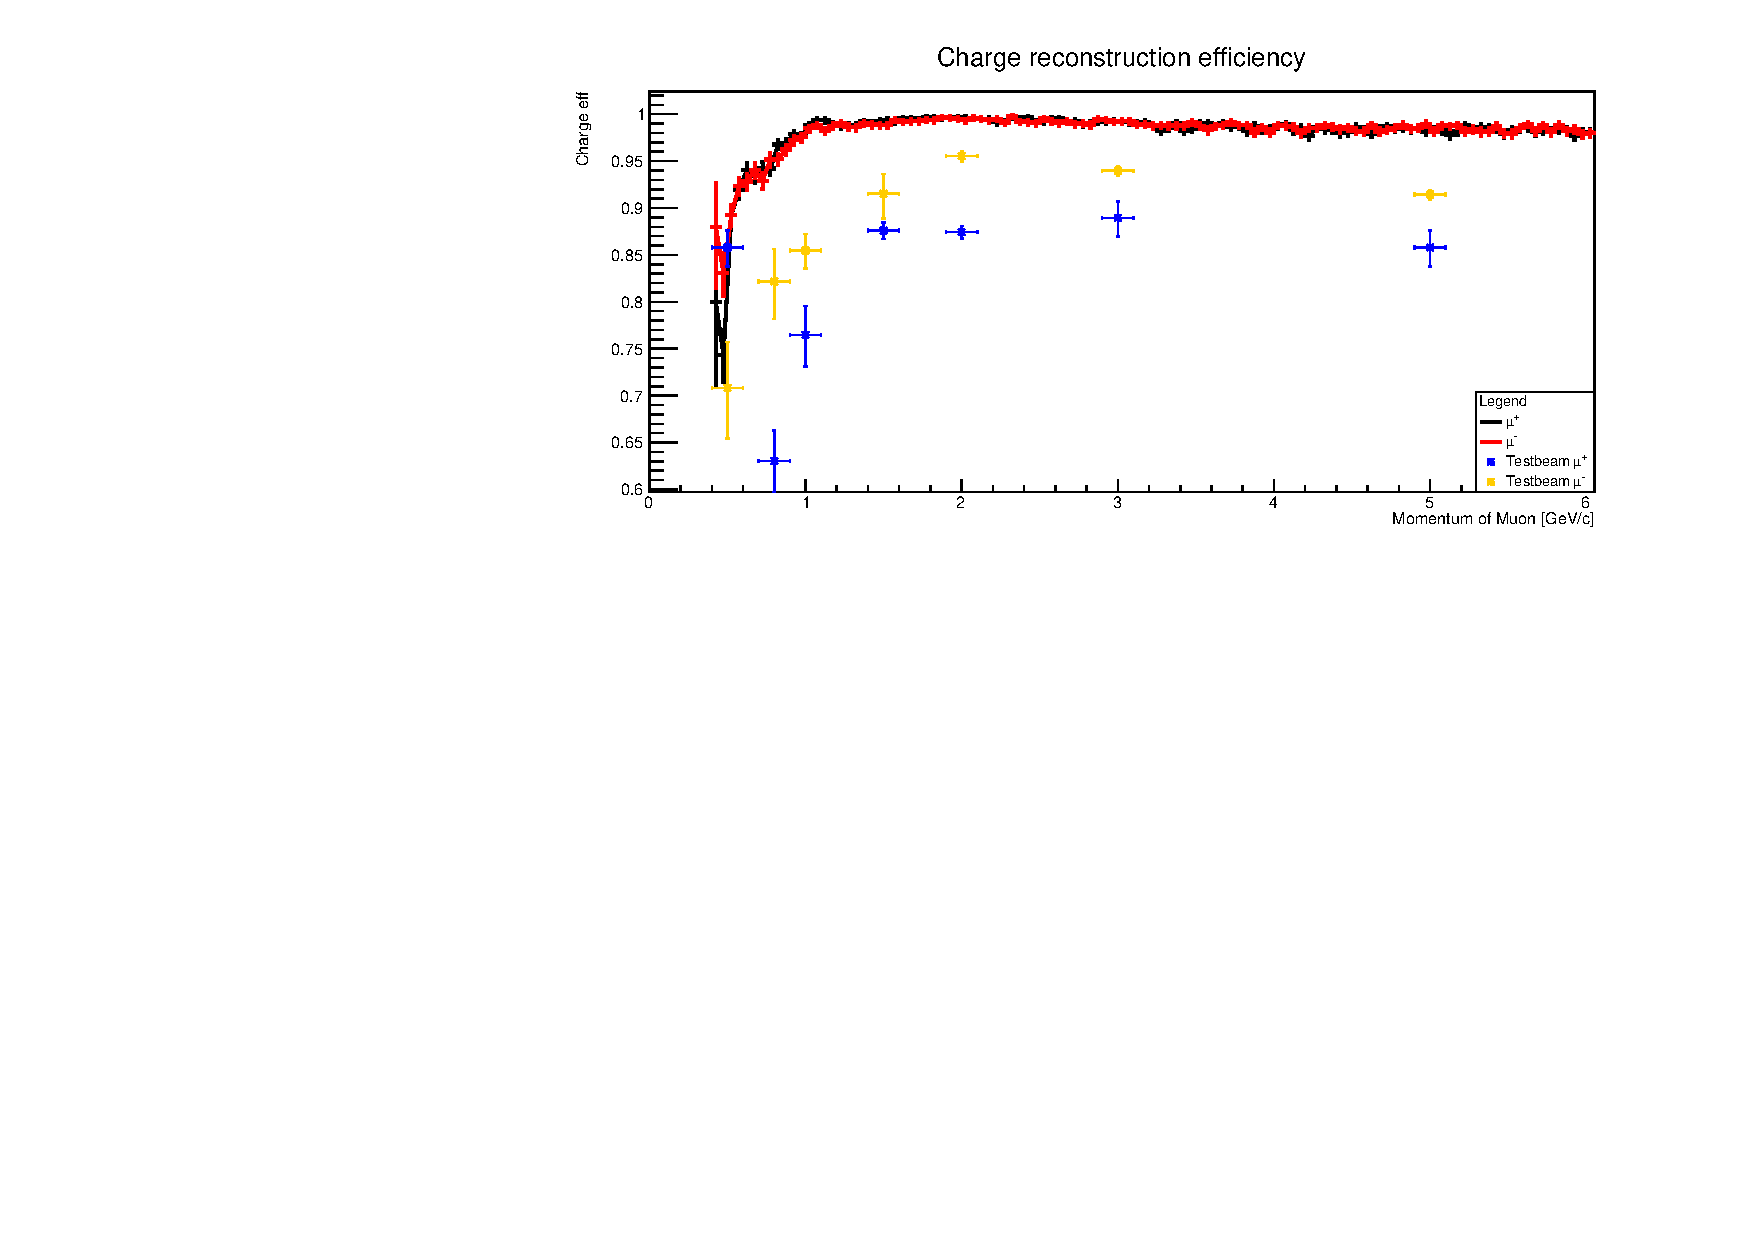
\includegraphics[width=\textwidth]{figures/testbeam/TestBeam090318Plots/ChargeIDFull6GeV.pdf}
%{figures/oldStudies/newChargeZoom5.pdf}

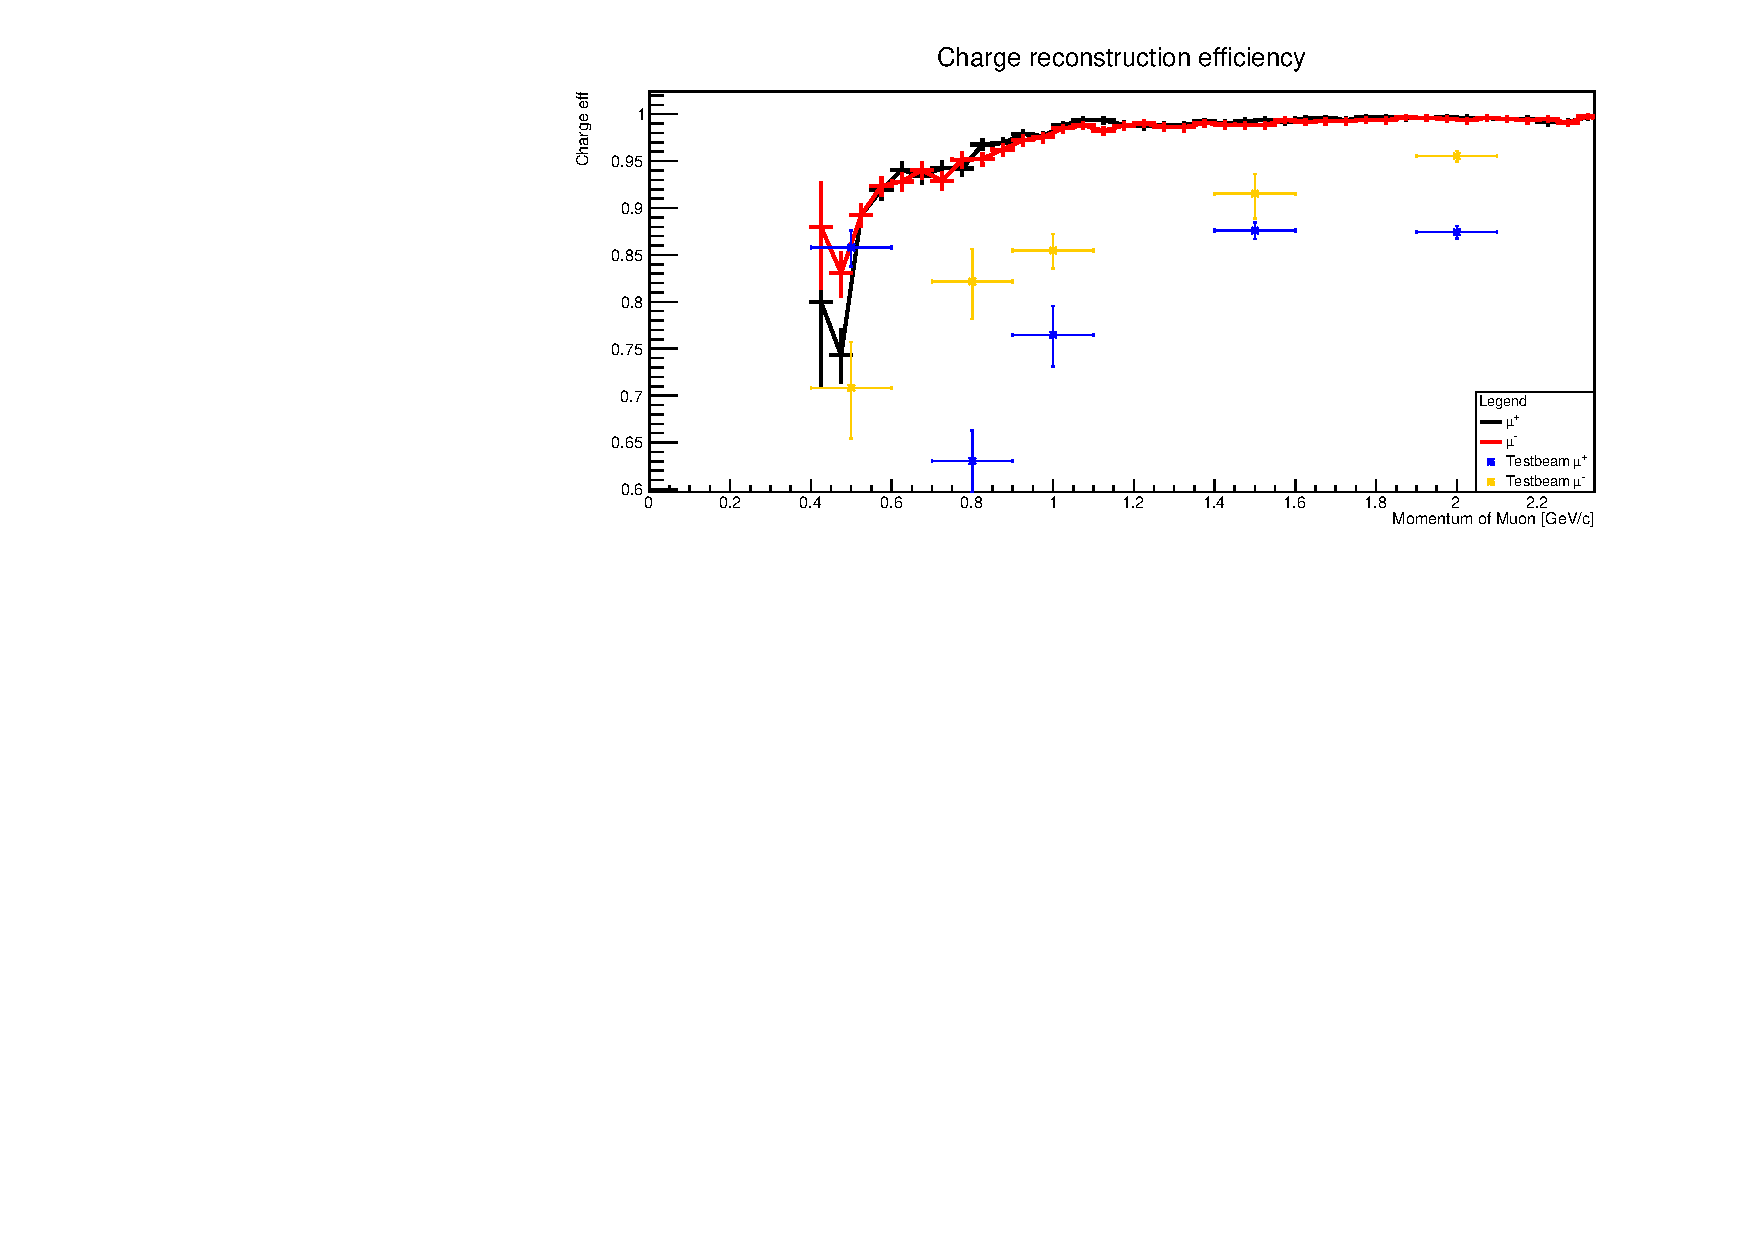
\includegraphics[width=\textwidth]{figures/testbeam/TestBeam090318Plots/ChargeIDFullLow.pdf}
%{figures/oldStudies/newChargeZoom1.pdf}


\caption{Initial charge id results}
\label{fig:ChargeInitial}
\end{figure}

These plots confirm that the full data analysis chain works however the results are slightly less than expected from simulations. Looking on an event by event basis it become clear that the events are a mix of muons and pions even after an initial pattern recognition. This motivated the development of a more advanced pattern recognition algorithm using machine learning. It can be seen that a simulated pion sample, \FigRef{fig:ChargeImprovedPion}, will be very poorly reconstructed and can explain the difference between data and simulation in the mixed test beam.

It should be mentioned that for future runs the deposited energy will be available and will make the distinction between pion and muon easier.

%Initial results, with pion contamination and initial unpacking. Discuss issue with cuts. Assuming that all hits had hit amplitude, unpacking could not collate hits correctly. Confirm reconstruction even further. Will be able to properly run the code on the data.

\begin{figure}[h!]
\centering
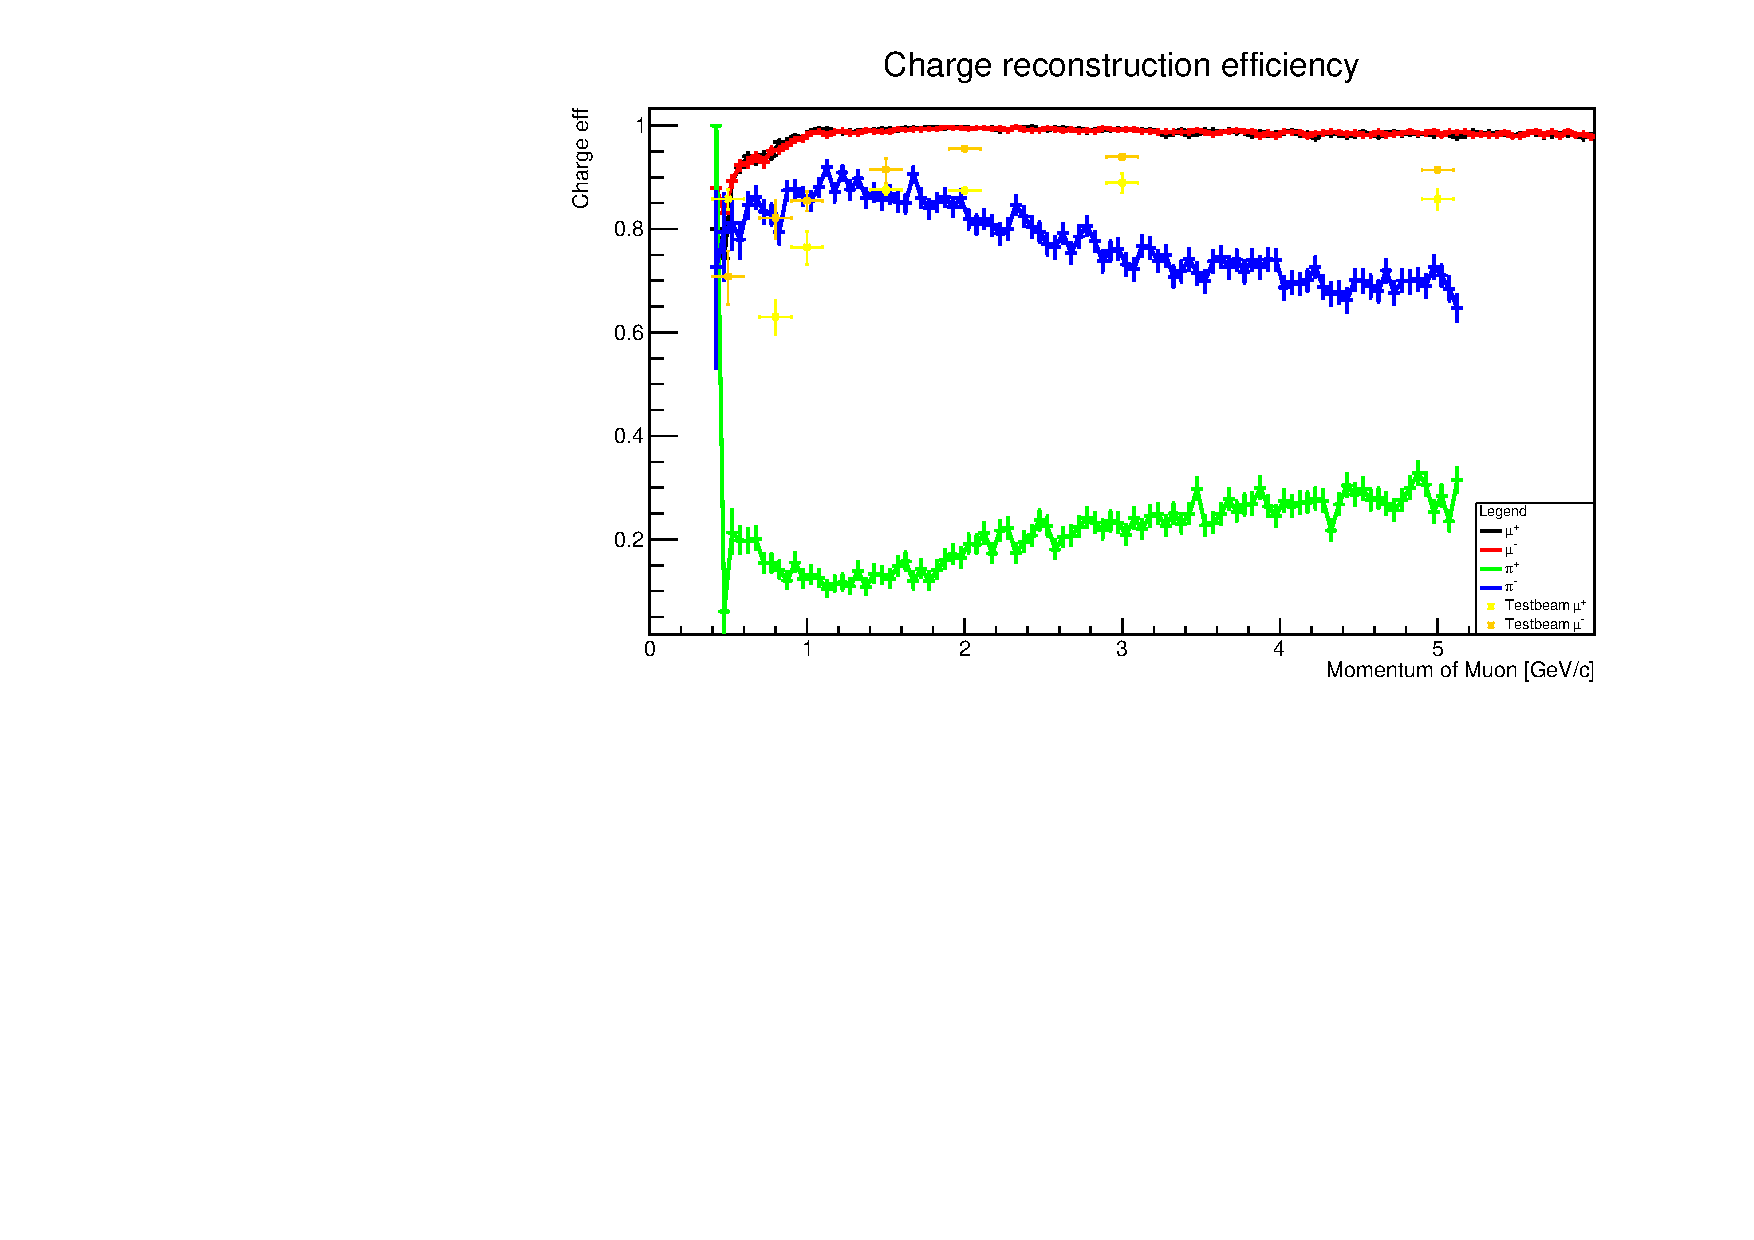
\includegraphics[width=\textwidth]{figures/testbeam/TestBeam090318Plots/ChargeIDFullWPion.pdf}

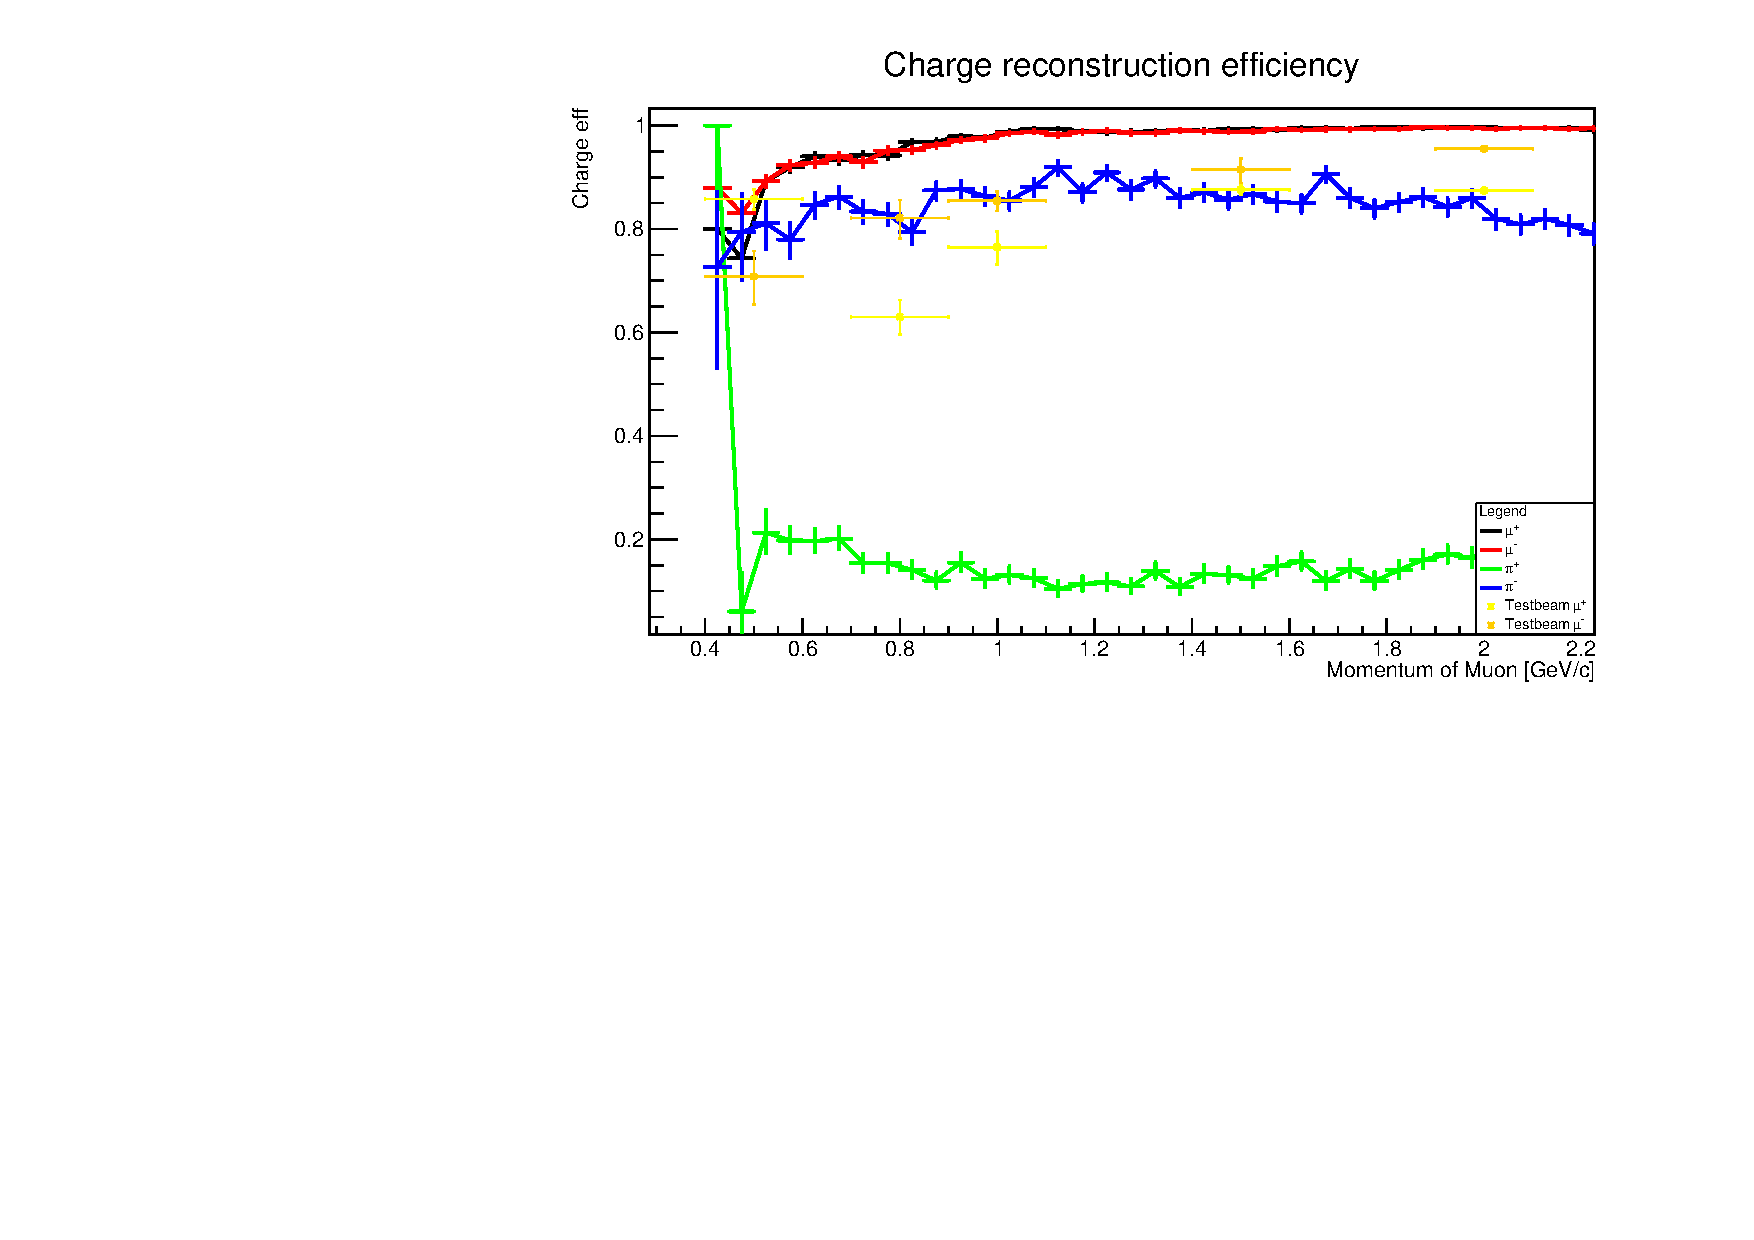
\includegraphics[width=\textwidth]{figures/testbeam/TestBeam090318Plots/ChargeIDFullLowWPion.pdf}
\caption{Simulated charge id for different particles vs data points}
\label{fig:ChargeImprovedPion}
\end{figure}

%Add in event displays. Something to show both pion showers and muons. See expecting bending for first time! enough data to test recpack! Low pt and recpack ! Different regions. Different run number? no real difference. Improved unpacking gave more data.


%Use pion data to show how it may be possible that it is contamination. Charge ID for pion is low, reconstruction eff is also poor.

%Reconstruction is defined as number of possible tracks in the software (more than 4 hits that produce a line) over tracks with a reconstructed momentum in the range $>0 and <\pm 10000$ i.e. a reasonable momentum. Charge takes these tracks and then checks charge.

%Charge ID study momentum reconstruction. look at charge id for particles correctly momentum reconstructed, look after TMVA pID. 


%Add details, not understanding what is correct data, further study has been performed but not solved problem efficiently. Unknown beam composition.

%\pagebreak
\clearpage
\subsubsection{Particle identification}
To further charge reconstruction, a  particle identification algorithm was developed using TMVA~\cite{TMVA} to classify muon from other events which may still pass through harsh criteria. The model has been developed to not be dependent on the momentum of the particle, should work for full range.

Essentially the machine learning algorithm identifies muons in a mixed background, but does not identify any particles in the background. This could be a future study and could be used to identify pions as well. In a more formal structure the signal is muons and the background are all of the remaining particles in the beam such as pions, protons etc.

The main variables used in the model are the following:
\begin{itemize}
\item Number of total hits,
\item Number of used planes for fit
\item Number of hits used for fit/ number of used planes
\item Average number of hits per plane
\item Maximum distance between hits in an event / Naive track length
\end{itemize}

These variables can be seen in \FigRef{fig:TMVAinput}.

\begin{figure}[h!]
\centering

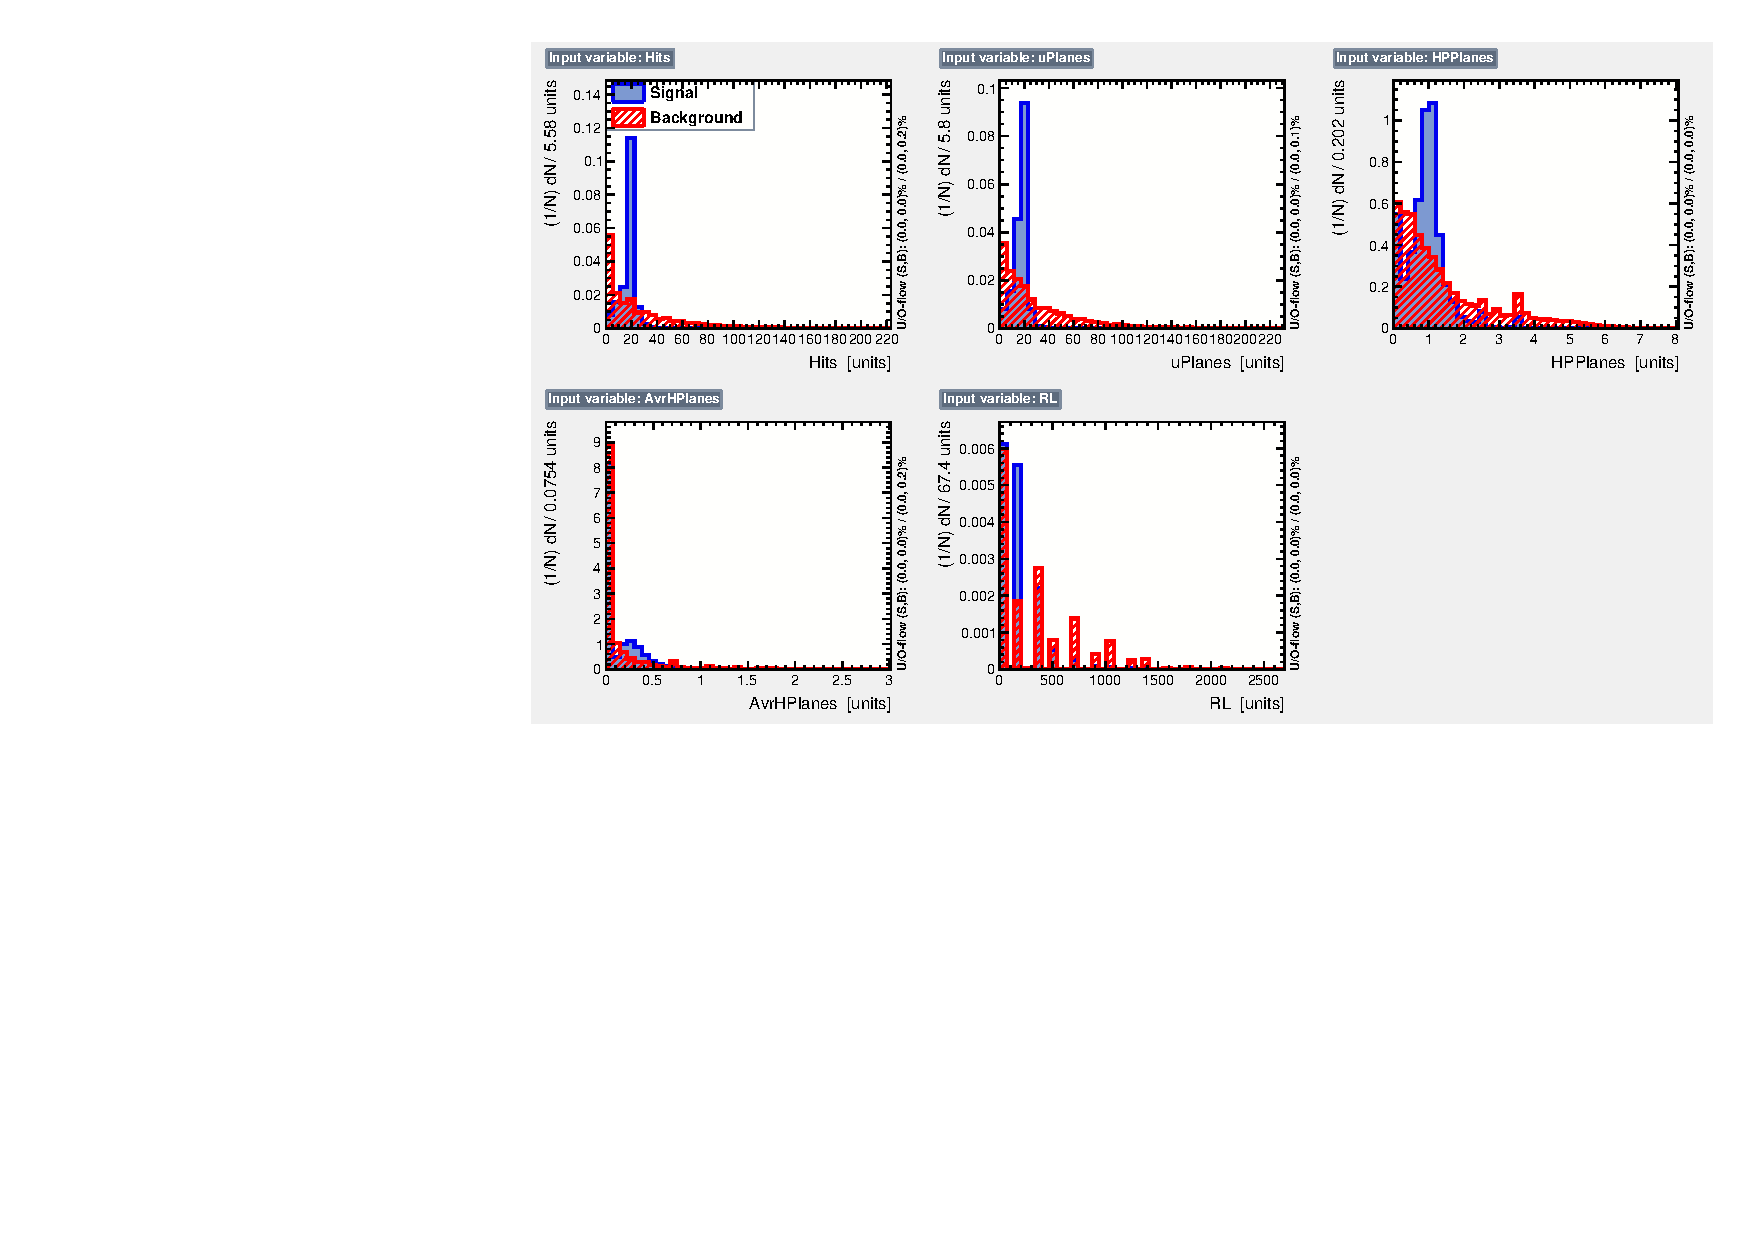
\includegraphics[width=\textwidth]{figures/TMVA/inputvariables.pdf}
\caption{Input variables for both signal and background using simulated data}
\label{fig:TMVAinput}
\end{figure}

Based on these simulated signal and background samples, TMVA will provided a Signal efficiency curve based on the various build in models, seen in \FigRef{fig:TMVAroc}. In this plot is is clear that several models outperform others, however the multilayer perception with a Bayesian Neural Network (MLPBNN) was choose as the best performing model. The specific performance can be seen in \FigRef{fig:TMVAroc2}.


%Currently found that the best method, however many perform similarly, is MLPBNN, Multilayer perceptron (neutral network) with BFGS training method, similar to gradient decent or quasi-Newton method, and bayesian regulator.


\begin{figure}[h!]
\centering

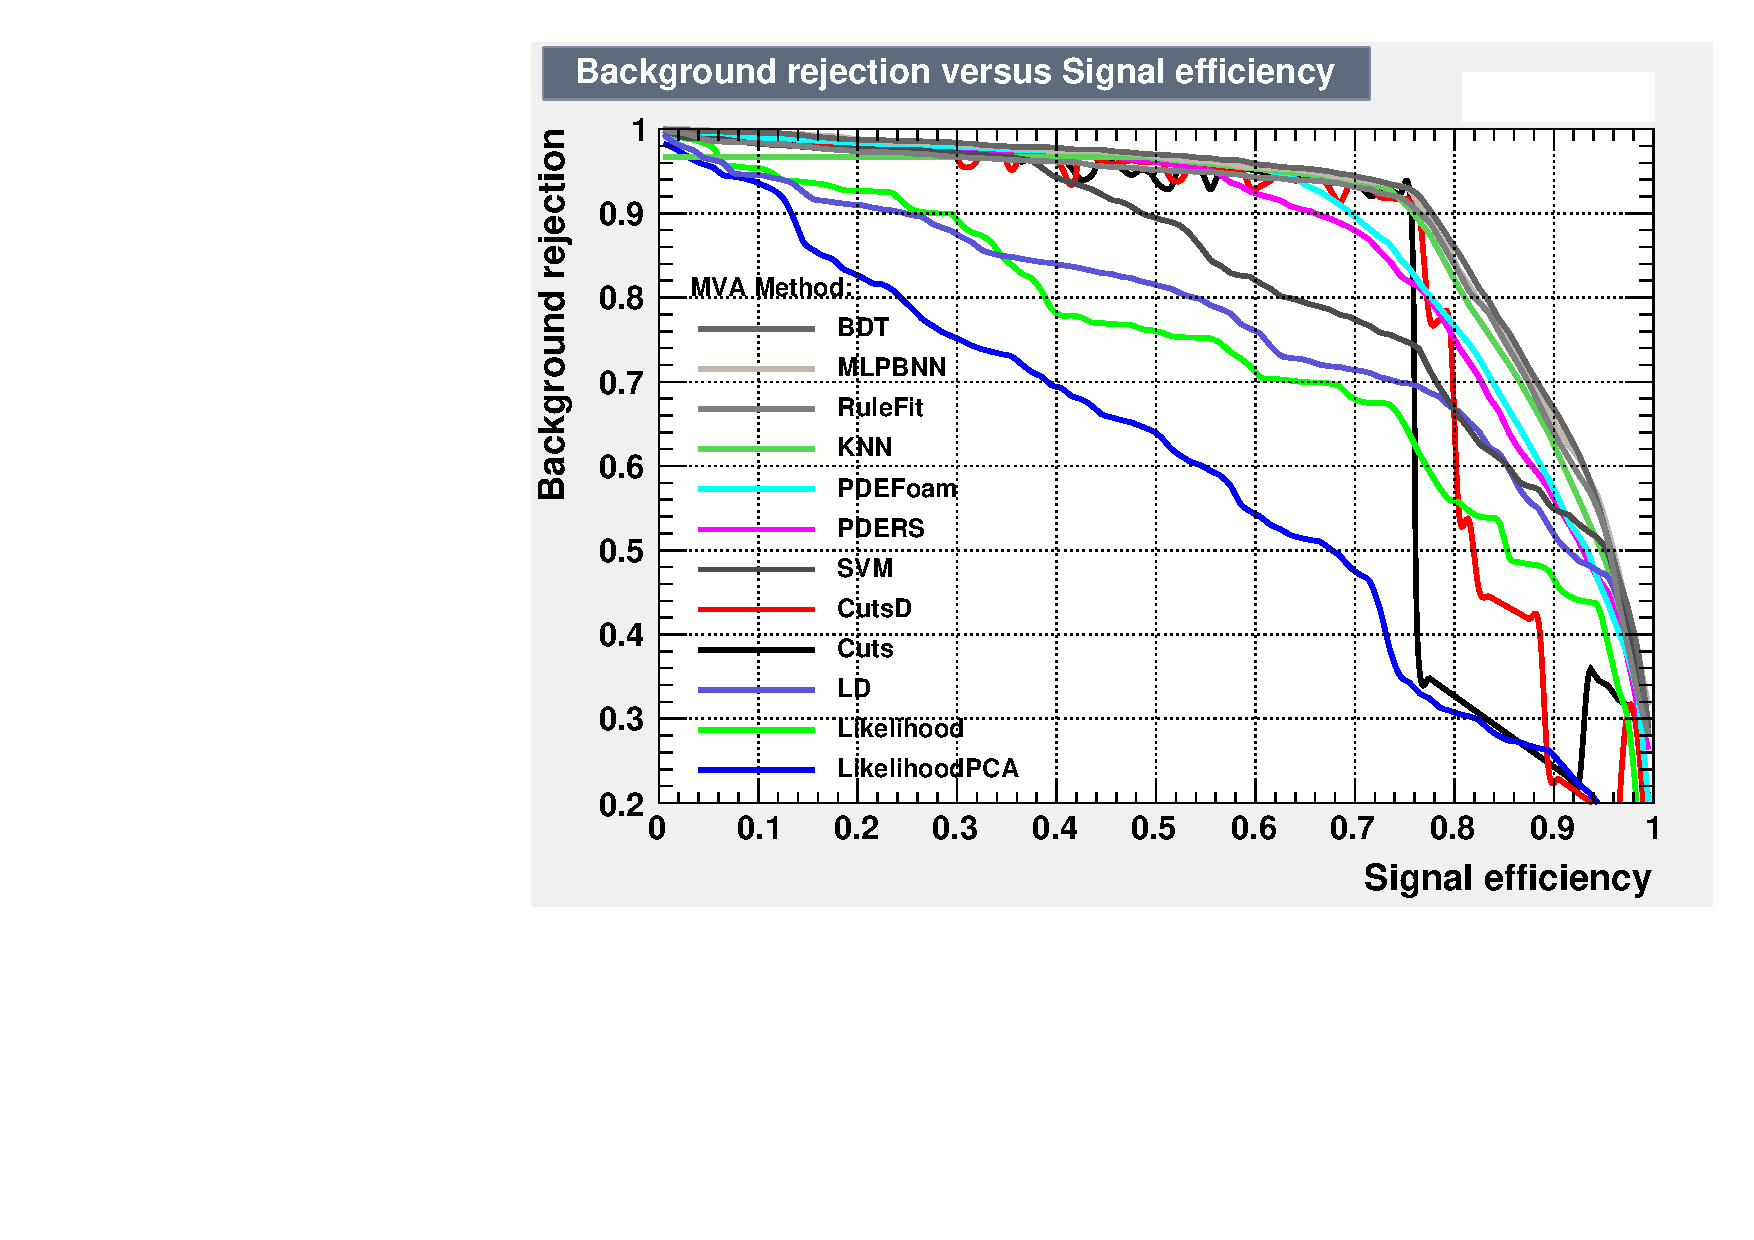
\includegraphics[width=\textwidth]{figures/TMVA/roc12.pdf}
\caption{ROC curve for various machine learning algorithms.}
\label{fig:TMVAroc}
\end{figure}

\begin{figure}[h!]
\centering

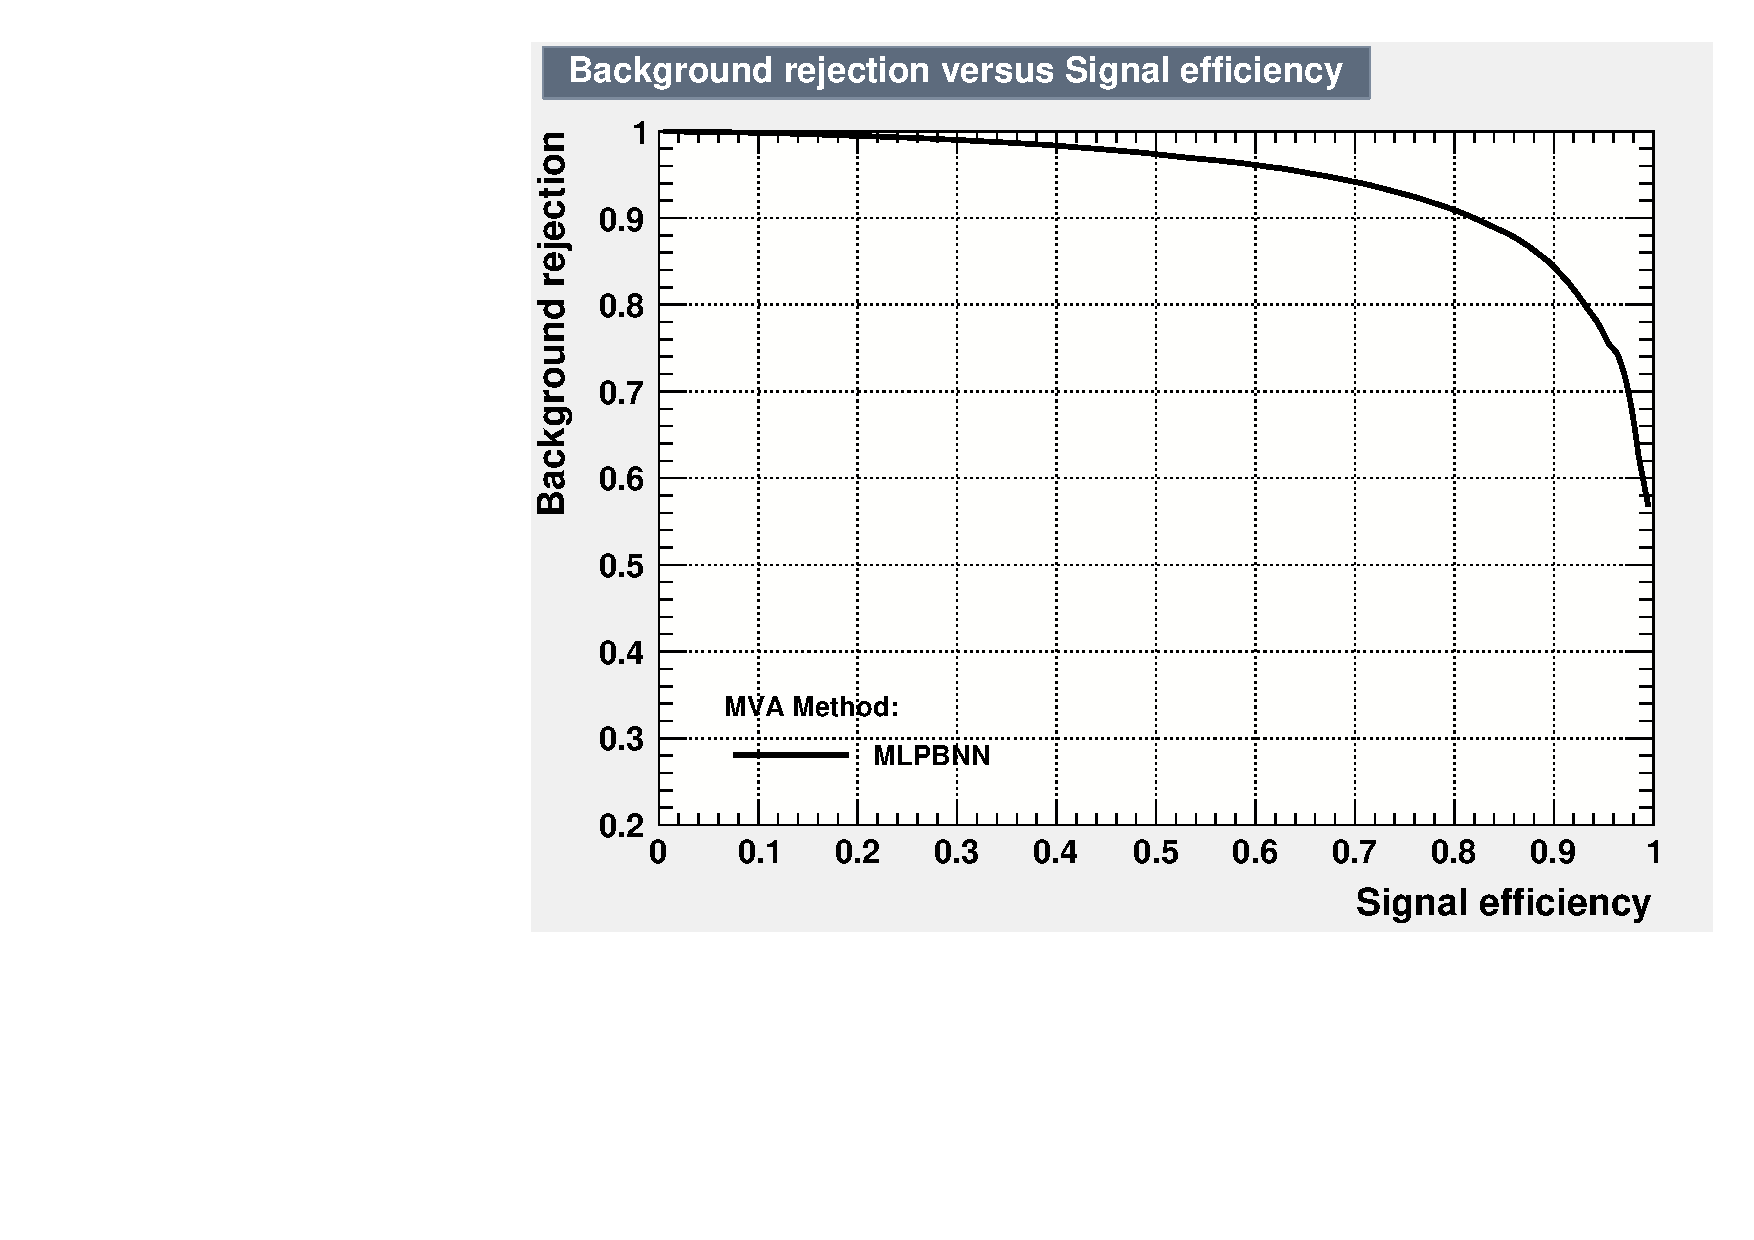
\includegraphics[width=\textwidth]{figures/TMVA/ROC1.pdf}
\caption{ROC curve for the chosen machine learning algorithms.}
\label{fig:TMVAroc2}
\end{figure}

Running through this model further it is possible to return the evaluation variable, known as the response to see how signal and background are classified by TMVA. Figure~\ref{fig:TMVAresponce} shows that signal and background can be separated and is understood by the algorithm, however there will always be some events which are incorrectly classified as signal or background. In the same figure it can be seen how data points have been added both by the training and testing sample to show that the algorithm has not been over-trained to work for only specific data.

This translates directly into \FigRef{fig:TMVAcuts} showing what value the of the response should be used to determine what is signal and background, providing a specific purity, efficiency and significance. For this analysis purity is of the most interest as the end goal is to return a data sample with as clean a muon sample as possible.

\begin{figure}[h!]
\centering
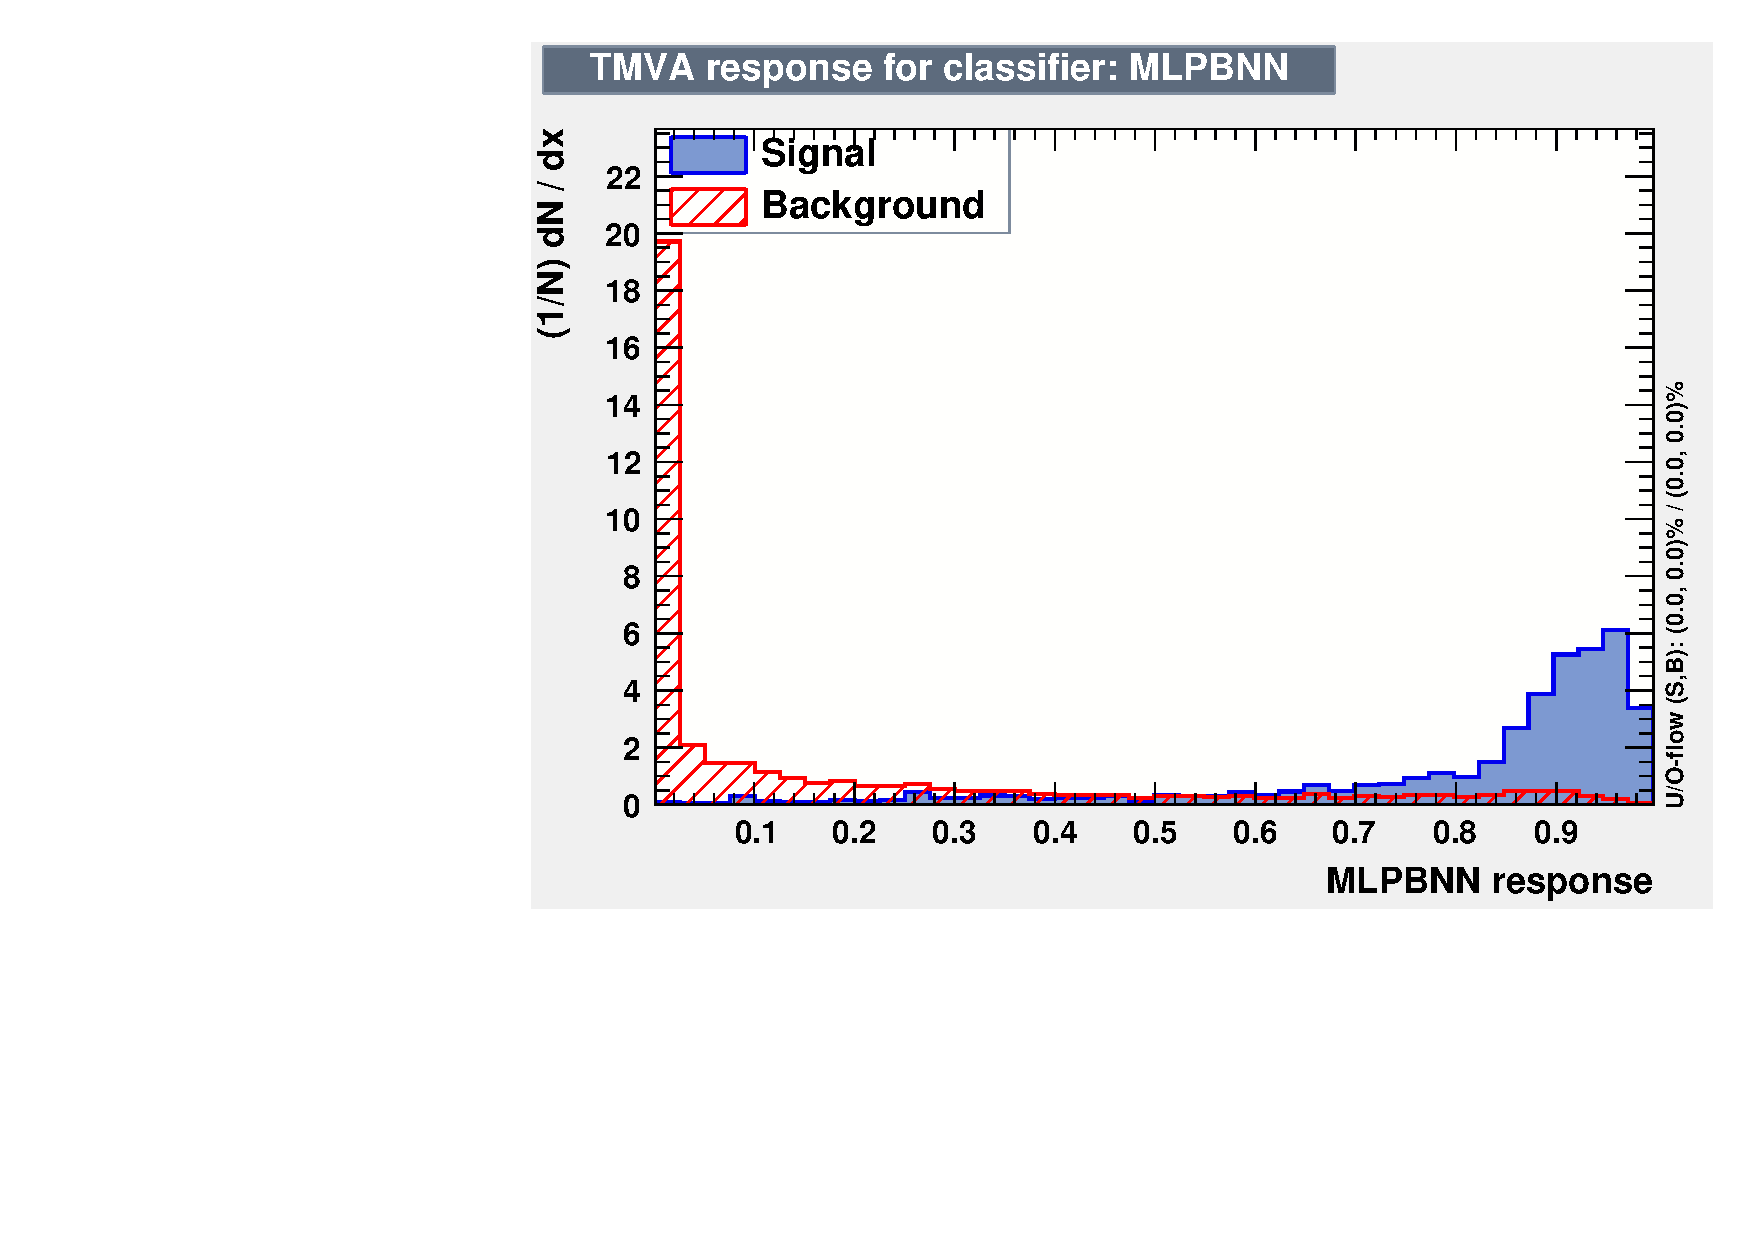
\includegraphics[width=.49\textwidth]{figures/TMVA/responceTest.pdf}
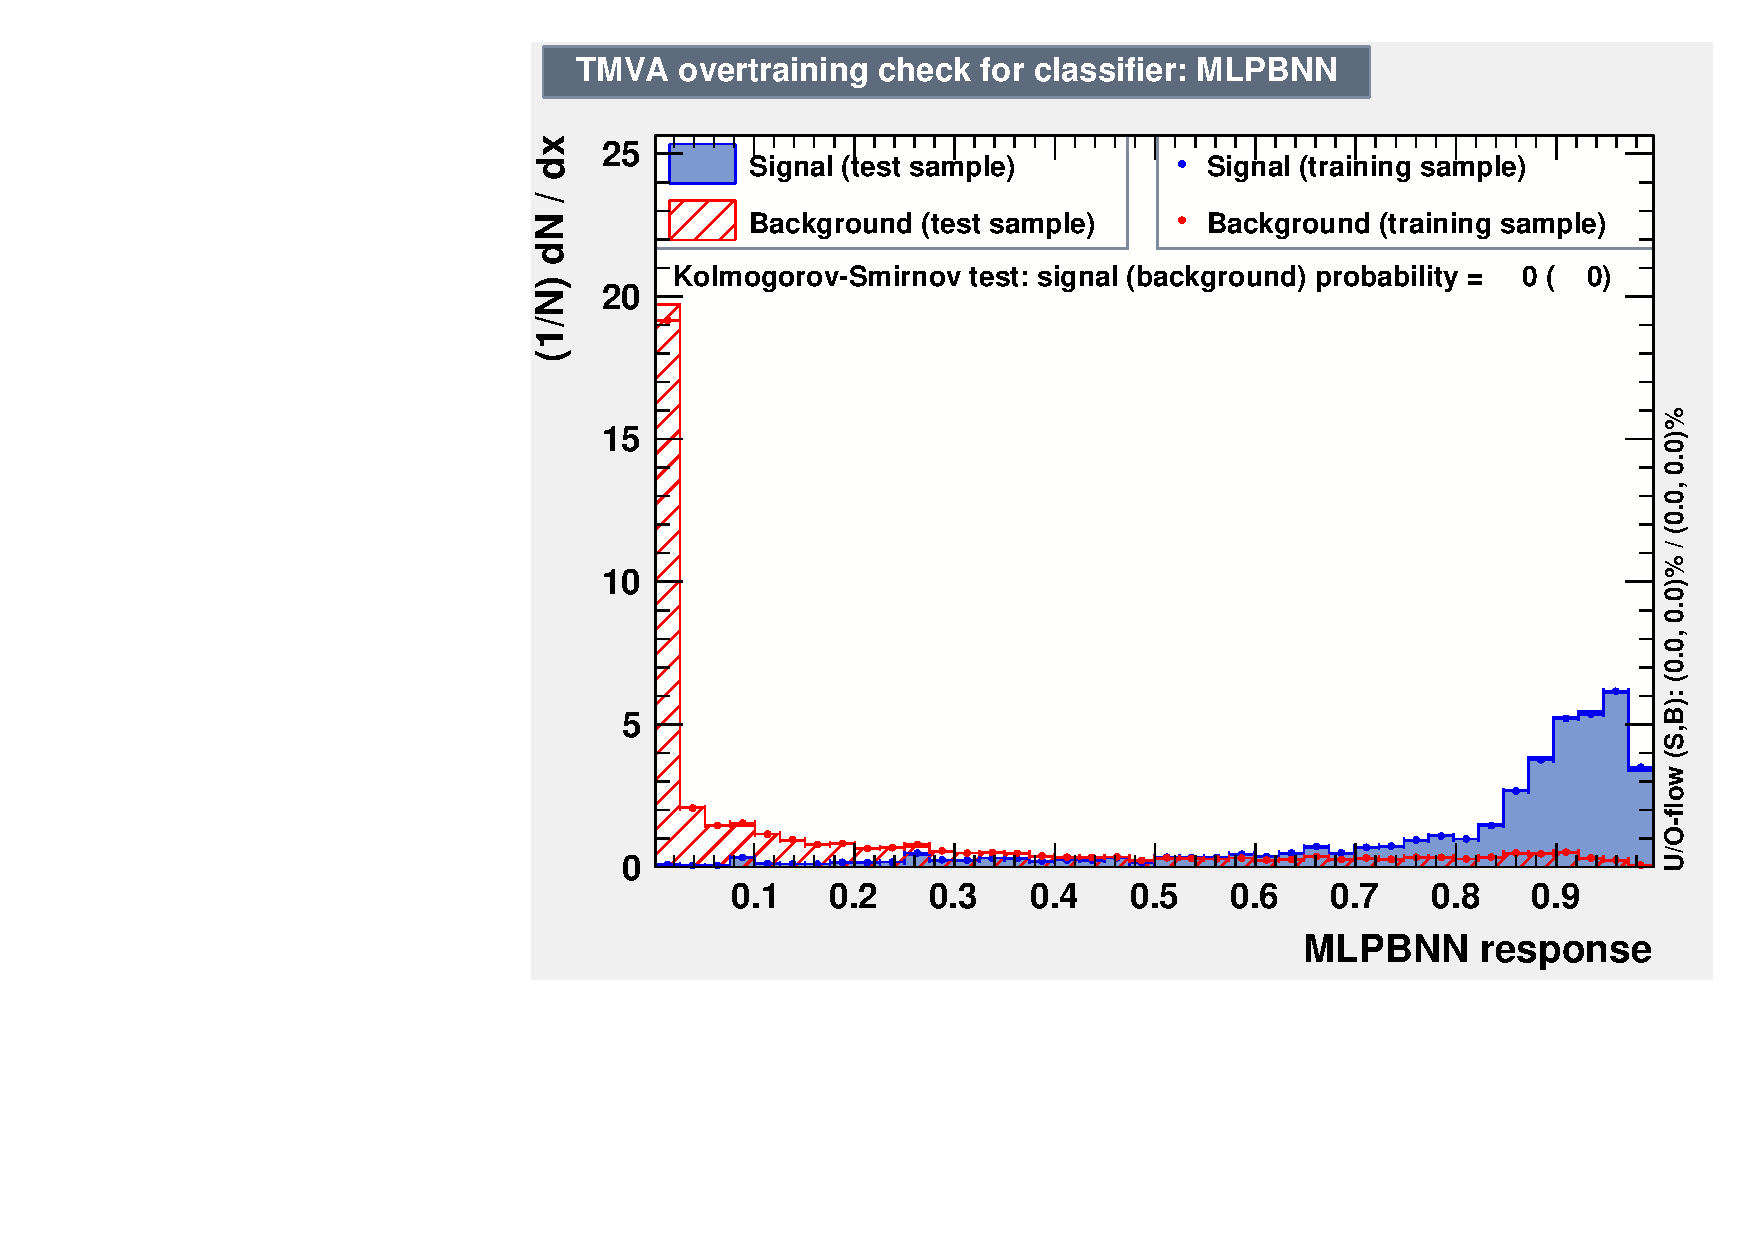
\includegraphics[width=.49\textwidth]{figures/TMVA/responceTestOT.pdf}
\caption{Responce with and without over-training check}
\label{fig:TMVAresponce}
\end{figure}

\begin{figure}[h!]
\centering

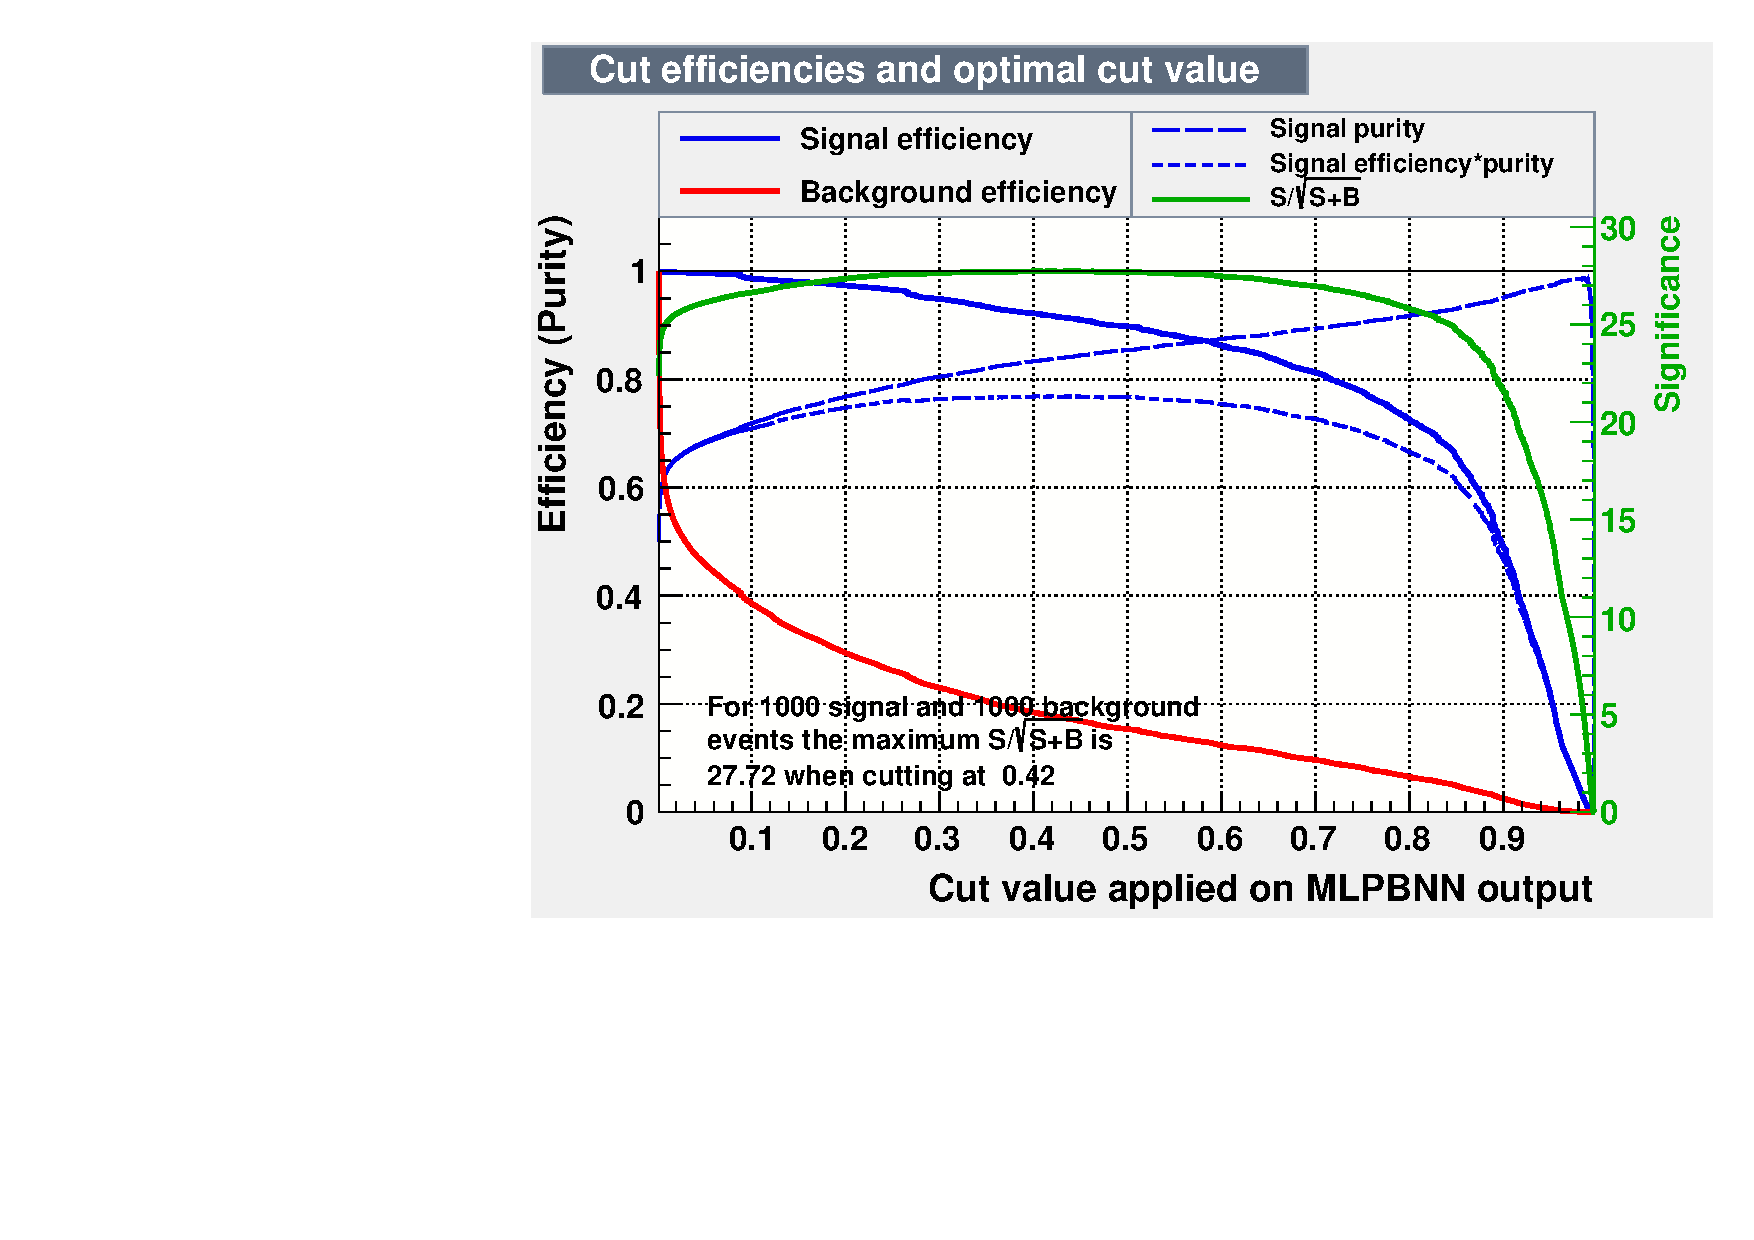
\includegraphics[width=\textwidth]{figures/TMVA/Cuts.pdf}
\caption{Cut efficiency plots.}
\label{fig:TMVAcuts}
\end{figure}

%What is this method? Cite the method? Show that many different methods would have produced very similar results.

%This also updates values provided from nufact and nuphys papers showing that the muon charge reconstruction is slightly lower than previously thought. it is still better than 0.6 previous MIND type experiments and show that it is possible to probe down to low energies which has not previously been shown.

%So far have results for $\mu^+/\mu^-$ in a background of  $\pi^+/\pi^-$. Will use for CCQE events compared to other neutrino interactions.

\clearpage
\subsubsection{Updated charge identification efficiency}

Using the final cleaned sample provides the final charge estimates as seen in \FigRef{fig:ChargeImproved}.

This finally shows, that assuming the beam after this is sufficiency pure there is a discrepancy between the simulations and final data representing detector and electronics factors which have not been taken into account. It should also be noted that the momentum values for the data are taken as the momenta selection set by the quadrupole magnets in the beam, which may not have been at the correct momentum value. This will require further study and potentially simulations of the entire beamline.

The plots show the potential of using a MIND type detector for muon charge reconstruction at lower momenta than than previously thought. It also shows that for the test beam it was possible of attaining above 70\% charge identification for the full momentum range and above 85\% for muons above 1 GeV/c. %The discrepancy between data and simulation is due to the act that the beam is not made up of purely muons as well as effects of the modelling of the electronics perhaps not taking all of the effects into account.

\begin{figure}[h!]
\centering
%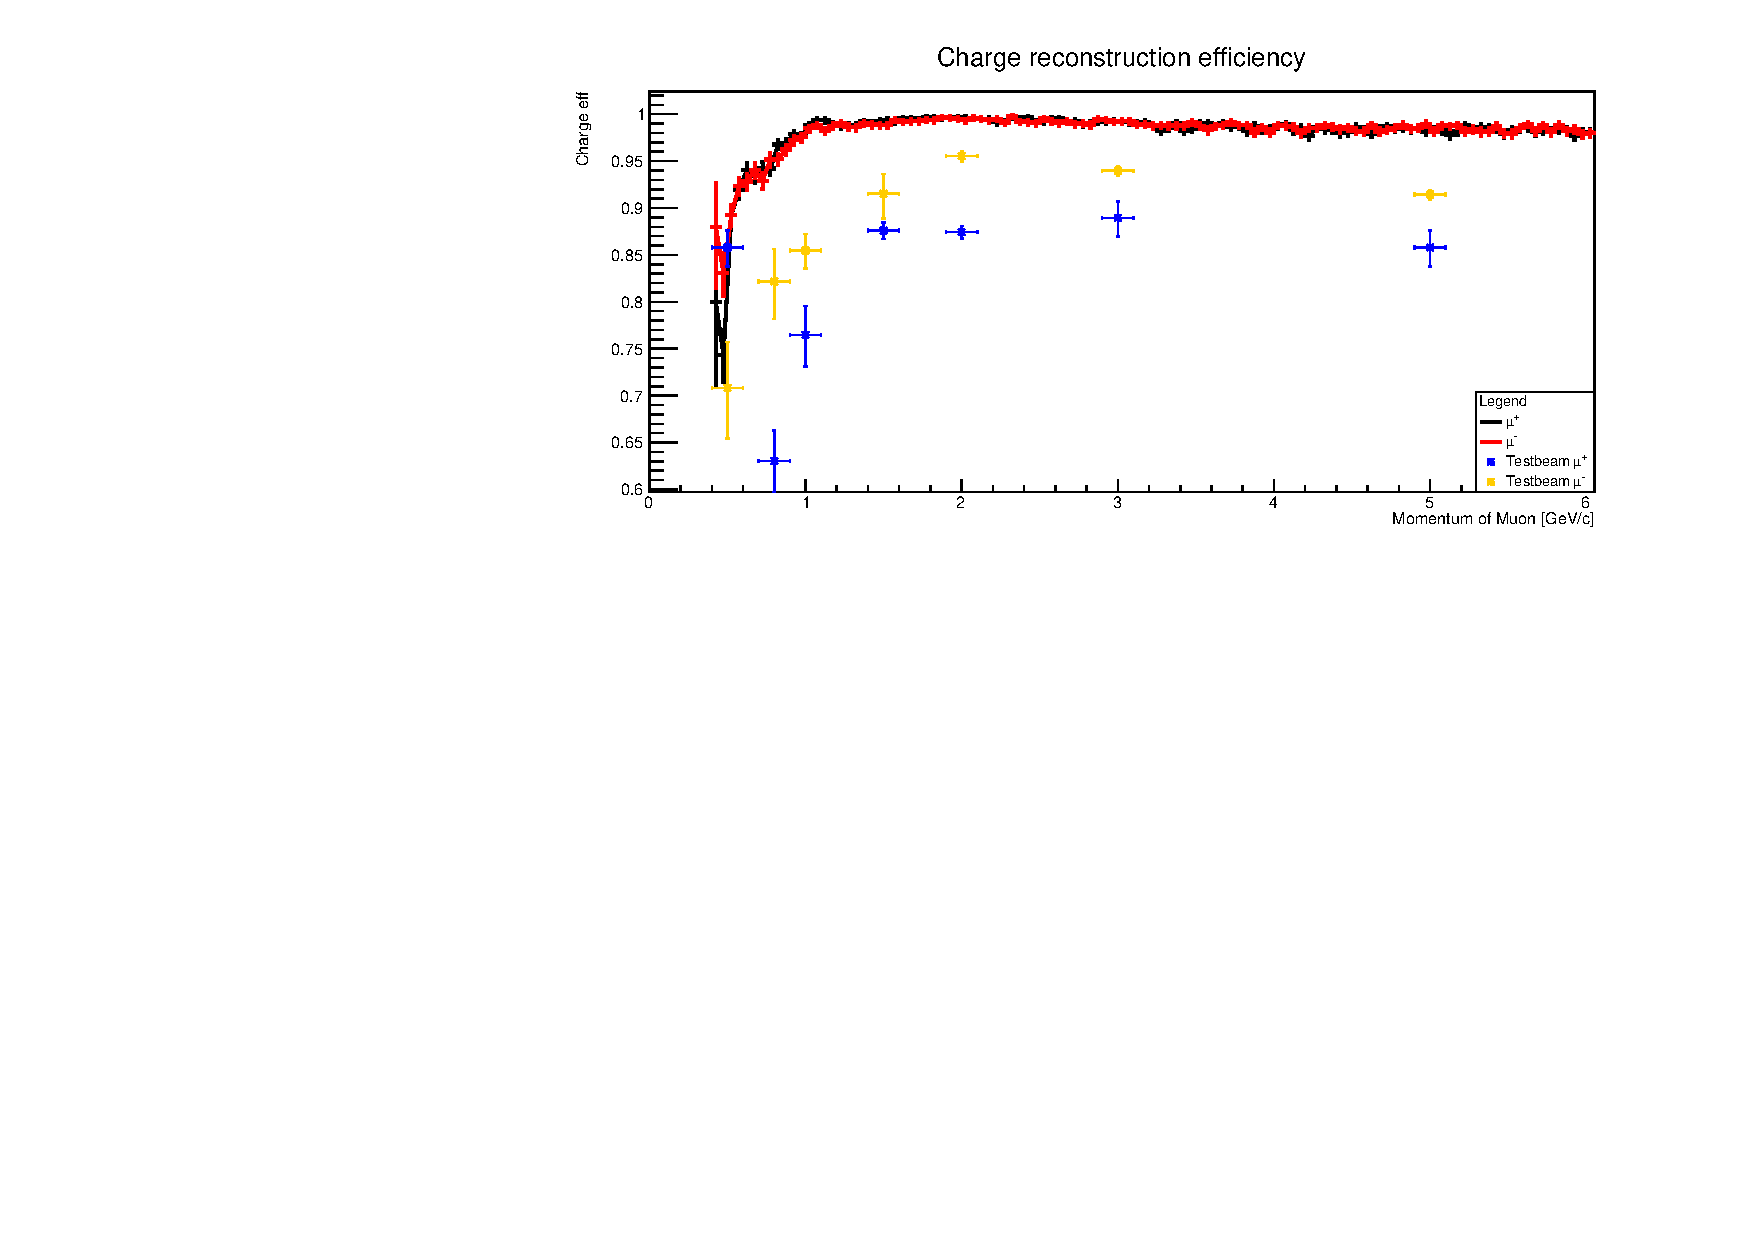
\includegraphics[width=0.49\textwidth]{figures/testbeam/TestBeam090318Plots/ChargeIDFull6GeV.pdf}
%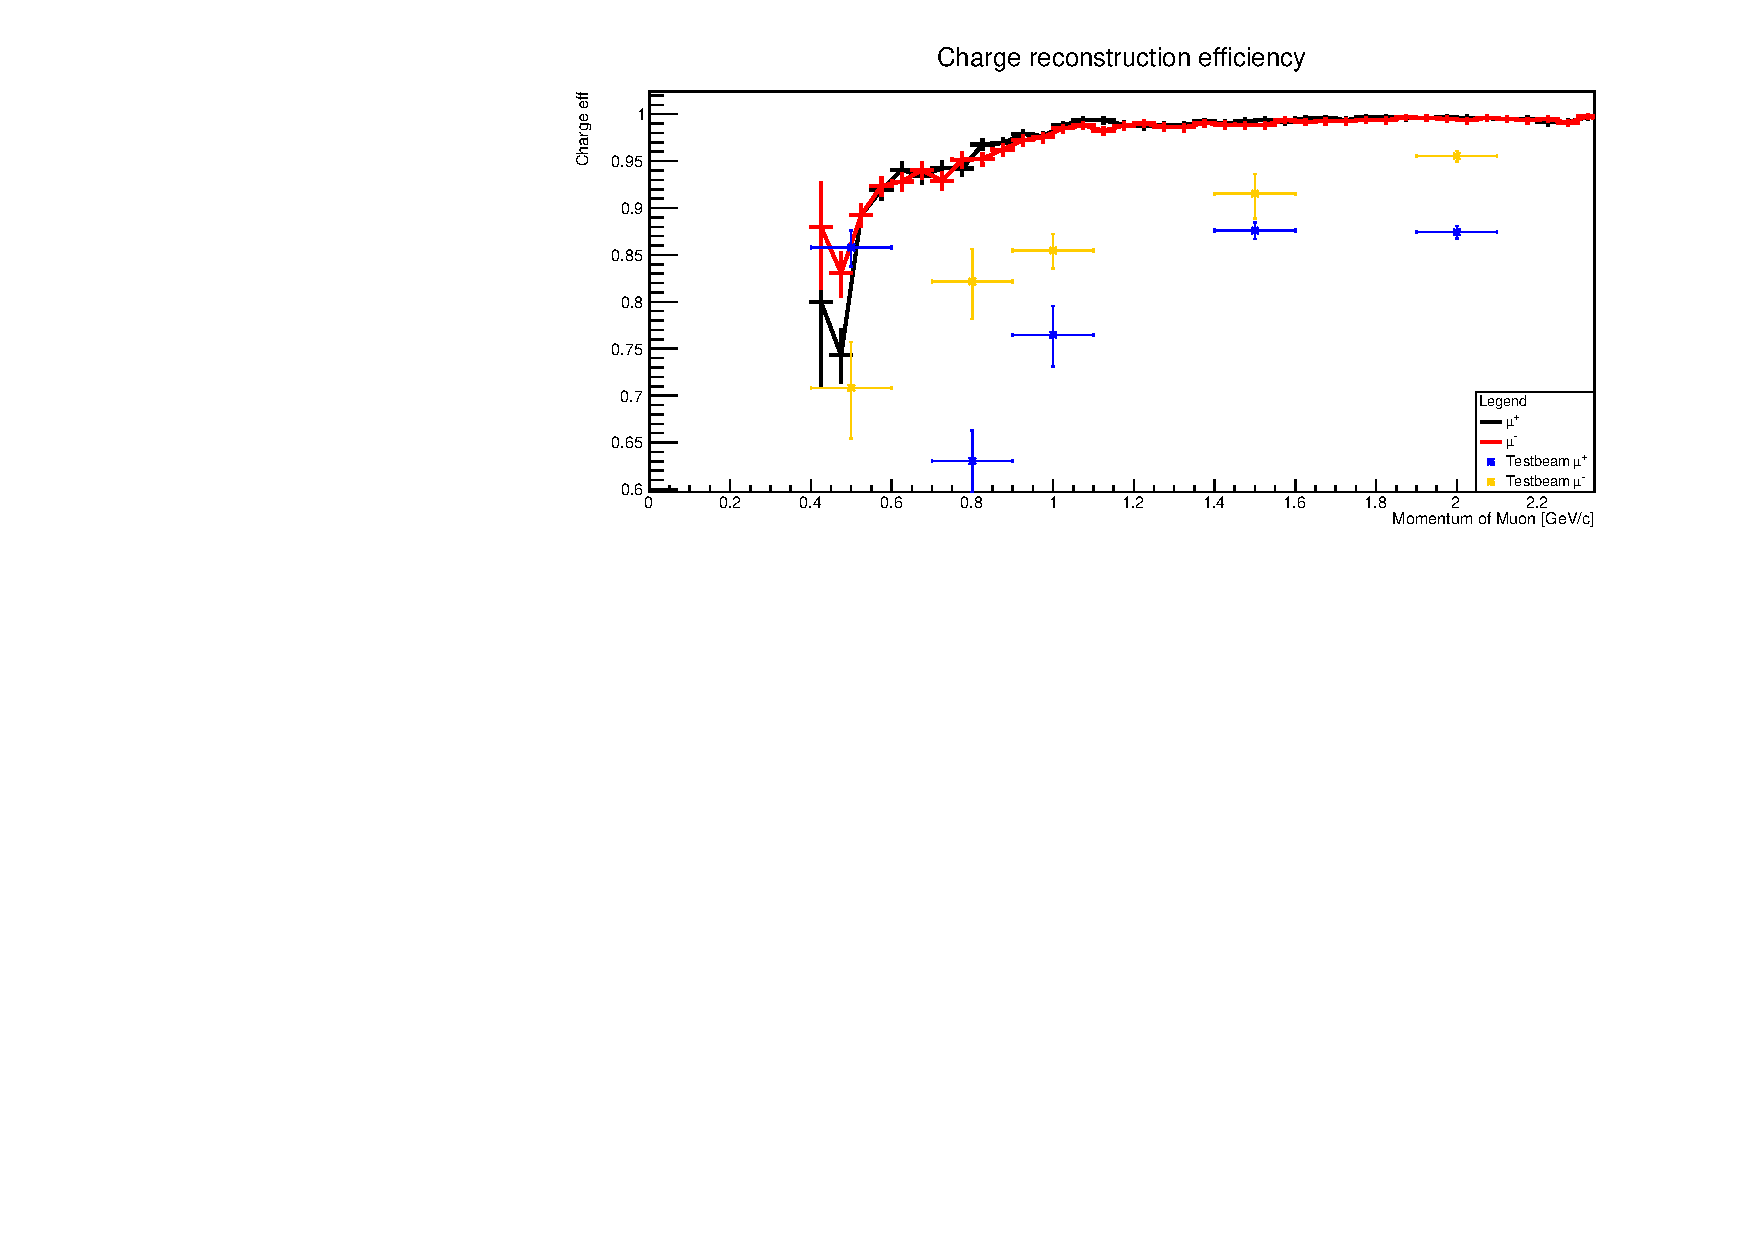
\includegraphics[width=0.49\textwidth]{figures/testbeam/TestBeam090318Plots/ChargeIDFullLow.pdf}

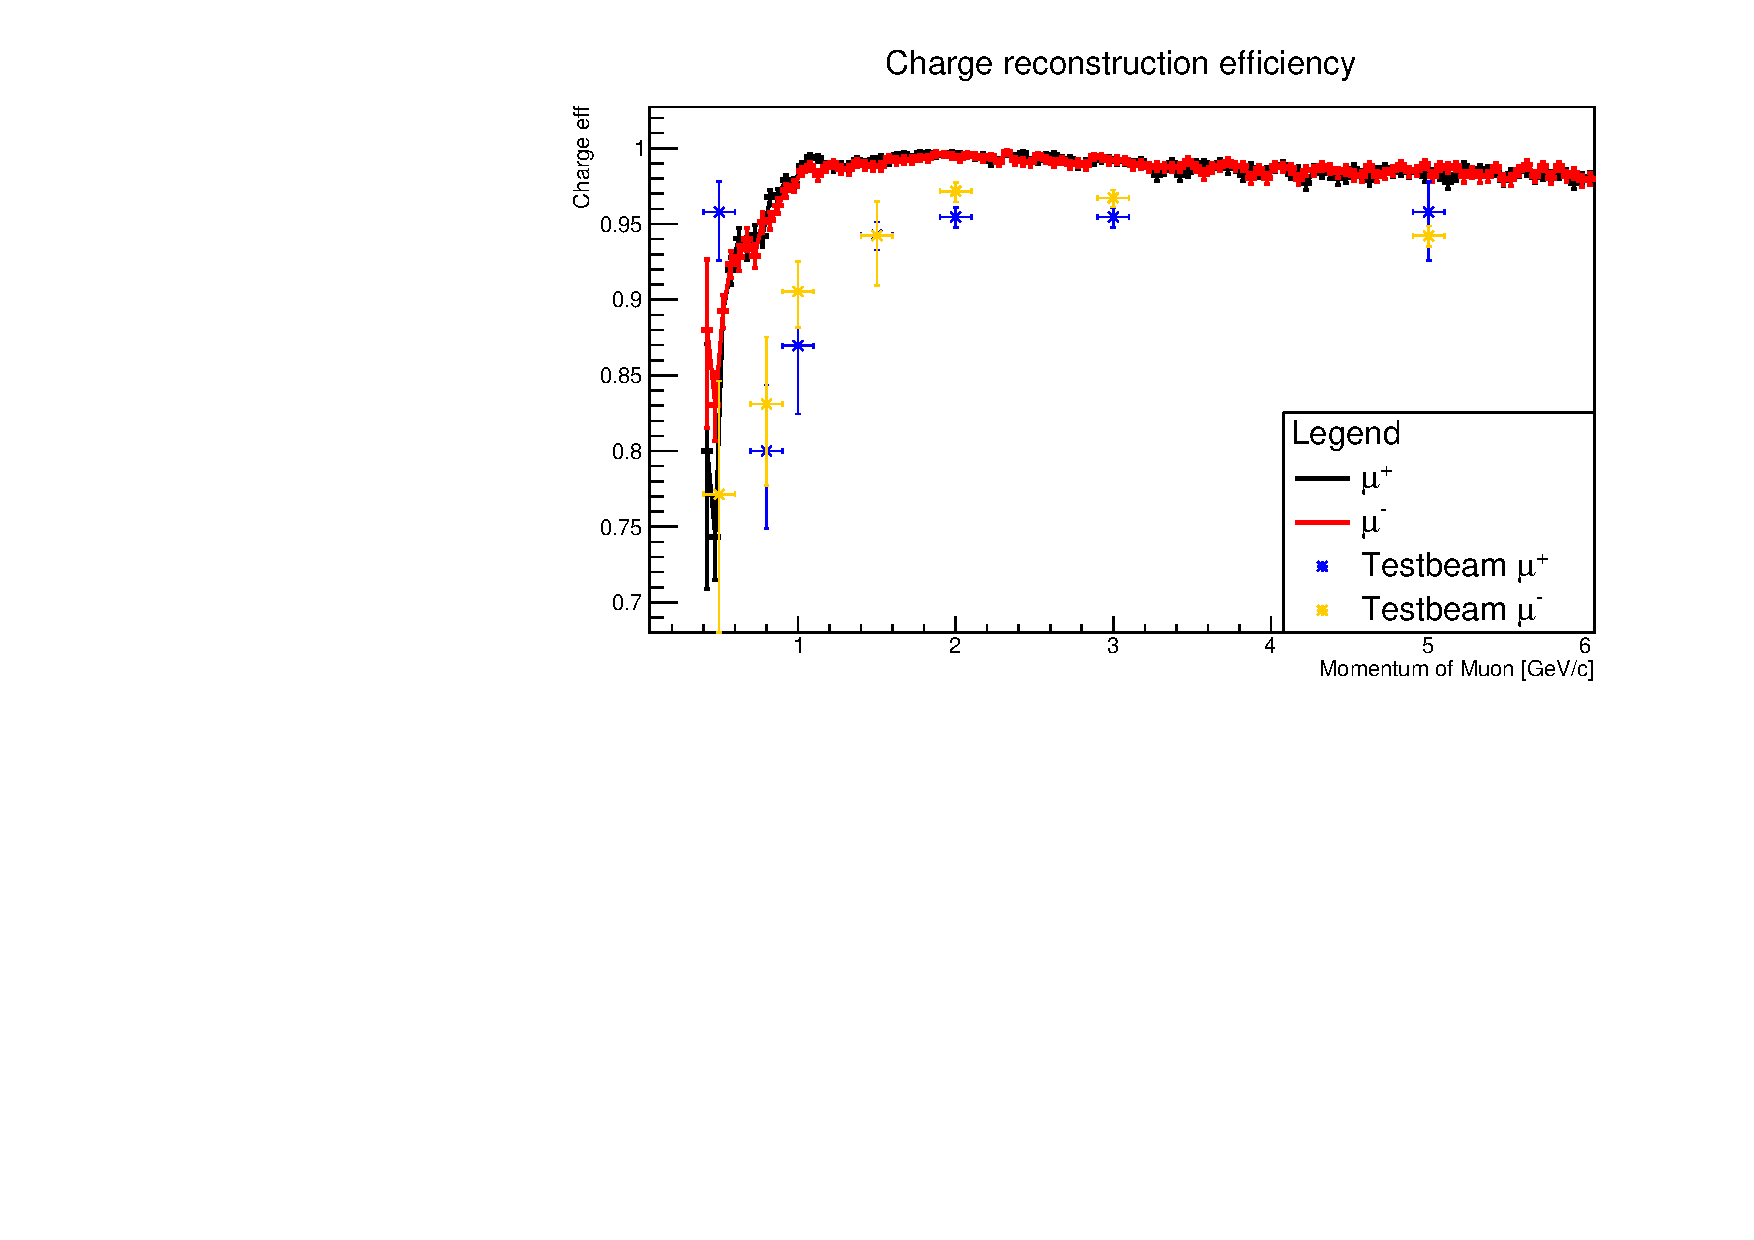
\includegraphics[width=\textwidth]
{figures/TMVAnew/TMVAnewChargeIDFull.pdf}%{figures/testbeam/TestBeam090318Plots/ChargeIDFull6GeV.pdf}

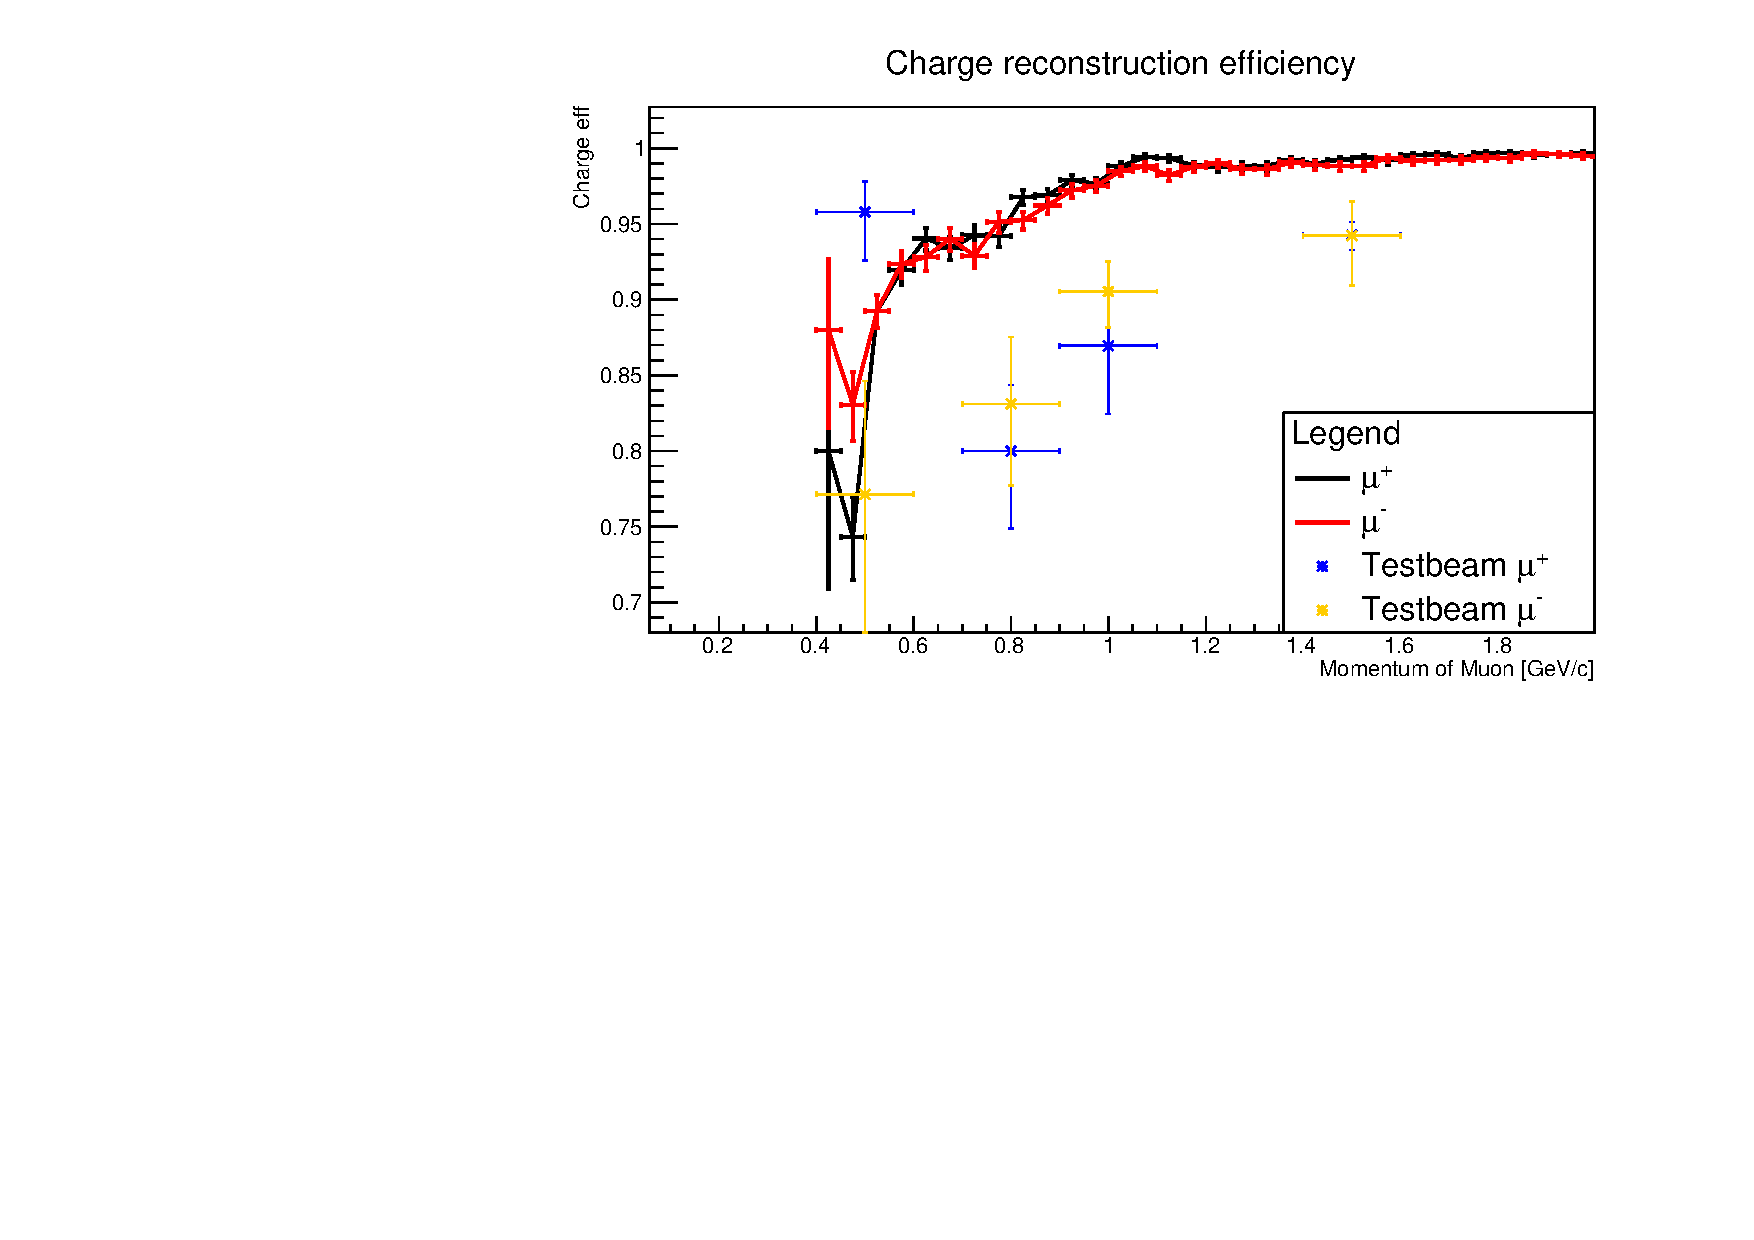
\includegraphics[width=\textwidth]{figures/TMVAnew/TMVAnewChargeIDLow.pdf}
%{figures/testbeam/TestBeam090318Plots/ChargeIDFullLow.pdf}

	%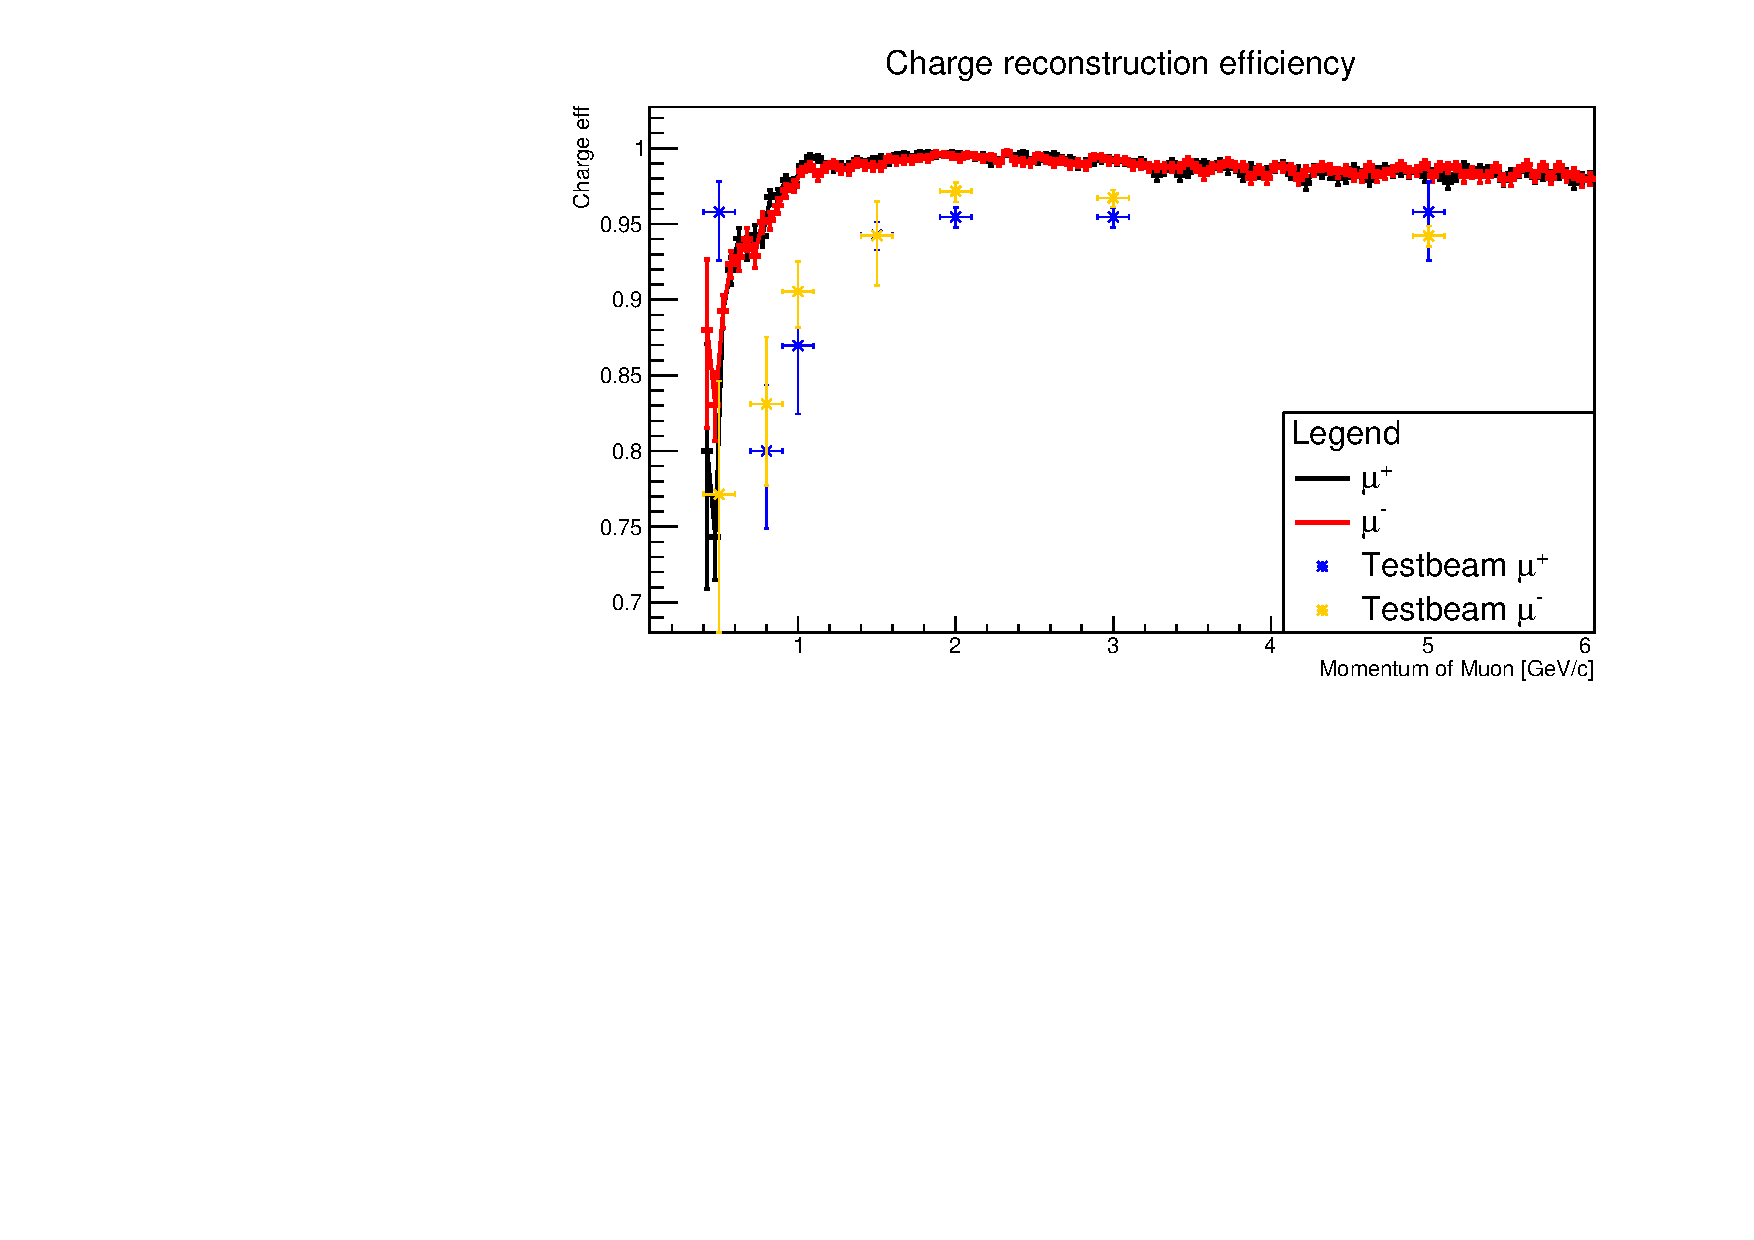
\includegraphics[width=0.49\textwidth]{figures/TMVAnew/TMVAnewChargeIDFull.pdf}
	%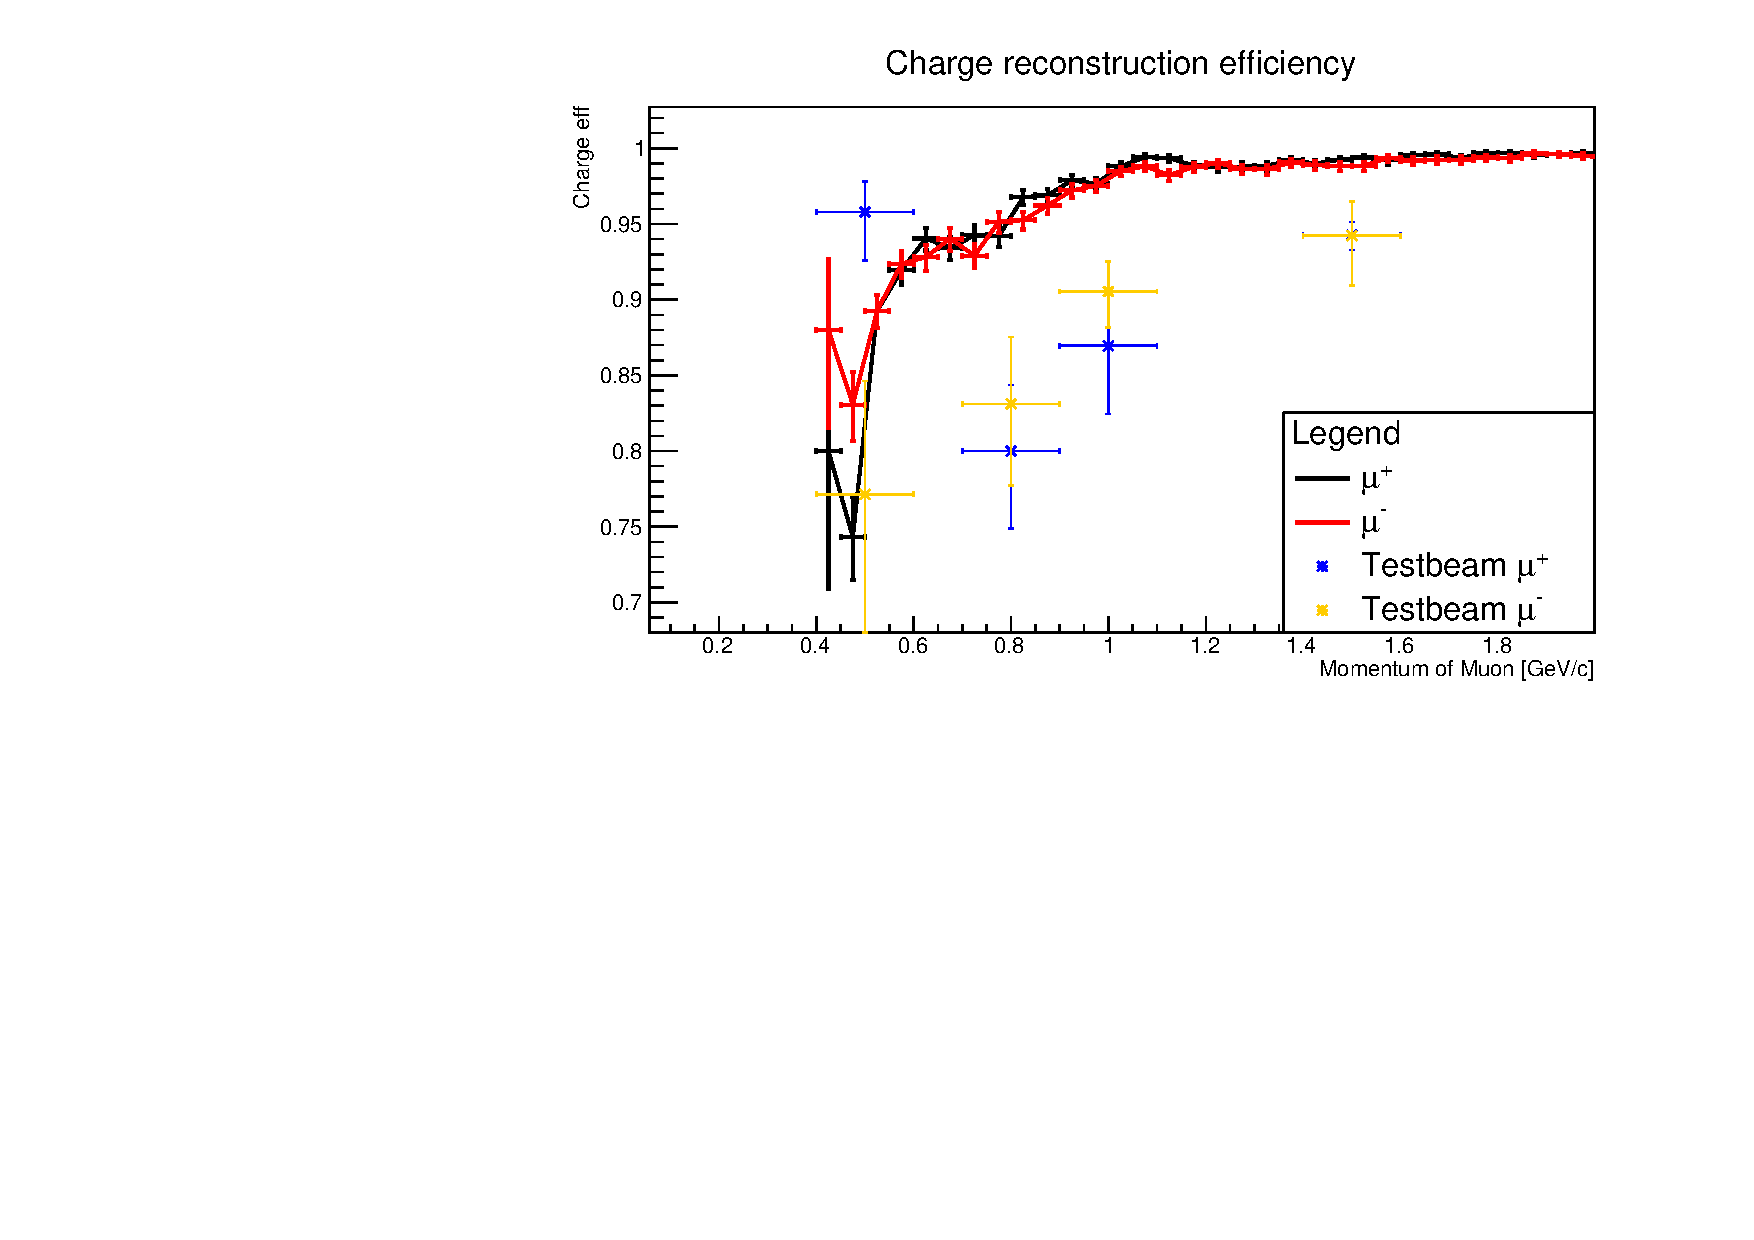
\includegraphics[width=0.49\textwidth]{figures/TMVAnew/TMVAnewChargeIDLow.pdf}

\caption{After TMVA charge id results}
\label{fig:ChargeImproved}
\end{figure}


%\subsubsection{Momentum reconstruction}
%Discuss results and show the spread and difference between expected (put in by hand) simulations and measured distributions. 

%Expected that the T9 beam area momentum is adjusted before final decay, actually choosing pion momentum and not muon momentum. Confirmed by email conversation. However, for lower momentum these match quite well. Large RMS from RecPack.

%Requires a new thinking regarding the reconstruction software and lead to the development of SAURON using more modern, reliable Kalman packages and a Runge-kutta method instead of a helical track model.

\section{Summary}
From the test beam it is clear that the Baby MIND performs as expected. The electronics works as well as the reconstruction in SaRoMaN, showing that charge identification is possible for muons at low momentum. The results how that the collaboration is ready to be integrated into the WAGASCI experiment for some neutrino data taking. 
